% Options for packages loaded elsewhere
\PassOptionsToPackage{unicode}{hyperref}
\PassOptionsToPackage{hyphens}{url}
%
\documentclass[
  english,
  man,floatsintext]{apa6}
\usepackage{lmodern}
\usepackage{amssymb,amsmath}
\usepackage{ifxetex,ifluatex}
\ifnum 0\ifxetex 1\fi\ifluatex 1\fi=0 % if pdftex
  \usepackage[T1]{fontenc}
  \usepackage[utf8]{inputenc}
  \usepackage{textcomp} % provide euro and other symbols
\else % if luatex or xetex
  \usepackage{unicode-math}
  \defaultfontfeatures{Scale=MatchLowercase}
  \defaultfontfeatures[\rmfamily]{Ligatures=TeX,Scale=1}
  \setmainfont[]{Helvetica}
\fi
% Use upquote if available, for straight quotes in verbatim environments
\IfFileExists{upquote.sty}{\usepackage{upquote}}{}
\IfFileExists{microtype.sty}{% use microtype if available
  \usepackage[]{microtype}
  \UseMicrotypeSet[protrusion]{basicmath} % disable protrusion for tt fonts
}{}
\makeatletter
\@ifundefined{KOMAClassName}{% if non-KOMA class
  \IfFileExists{parskip.sty}{%
    \usepackage{parskip}
  }{% else
    \setlength{\parindent}{0pt}
    \setlength{\parskip}{6pt plus 2pt minus 1pt}}
}{% if KOMA class
  \KOMAoptions{parskip=half}}
\makeatother
\usepackage{xcolor}
\IfFileExists{xurl.sty}{\usepackage{xurl}}{} % add URL line breaks if available
\IfFileExists{bookmark.sty}{\usepackage{bookmark}}{\usepackage{hyperref}}
\hypersetup{
  pdftitle={Convolutional neural networks can decode eye movement data: A black box approach to predicting task from eye movements},
  pdflang={en-EN},
  pdfkeywords={deep learning, eye tracking, convolutional neural network, cognitive state, endogenous attention},
  hidelinks,
  pdfcreator={LaTeX via pandoc}}
\urlstyle{same} % disable monospaced font for URLs
\usepackage{graphicx,grffile}
\makeatletter
\def\maxwidth{\ifdim\Gin@nat@width>\linewidth\linewidth\else\Gin@nat@width\fi}
\def\maxheight{\ifdim\Gin@nat@height>\textheight\textheight\else\Gin@nat@height\fi}
\makeatother
% Scale images if necessary, so that they will not overflow the page
% margins by default, and it is still possible to overwrite the defaults
% using explicit options in \includegraphics[width, height, ...]{}
\setkeys{Gin}{width=\maxwidth,height=\maxheight,keepaspectratio}
% Set default figure placement to htbp
\makeatletter
\def\fps@figure{htbp}
\makeatother
\setlength{\emergencystretch}{3em} % prevent overfull lines
\providecommand{\tightlist}{%
  \setlength{\itemsep}{0pt}\setlength{\parskip}{0pt}}
\setcounter{secnumdepth}{-\maxdimen} % remove section numbering
% Make \paragraph and \subparagraph free-standing
\ifx\paragraph\undefined\else
  \let\oldparagraph\paragraph
  \renewcommand{\paragraph}[1]{\oldparagraph{#1}\mbox{}}
\fi
\ifx\subparagraph\undefined\else
  \let\oldsubparagraph\subparagraph
  \renewcommand{\subparagraph}[1]{\oldsubparagraph{#1}\mbox{}}
\fi
% Manuscript styling
\usepackage{upgreek}
\captionsetup{font=singlespacing,justification=justified}

% Table formatting
\usepackage{longtable}
\usepackage{lscape}
% \usepackage[counterclockwise]{rotating}   % Landscape page setup for large tables
\usepackage{multirow}		% Table styling
\usepackage{tabularx}		% Control Column width
\usepackage[flushleft]{threeparttable}	% Allows for three part tables with a specified notes section
\usepackage{threeparttablex}            % Lets threeparttable work with longtable

% Create new environments so endfloat can handle them
% \newenvironment{ltable}
%   {\begin{landscape}\begin{center}\begin{threeparttable}}
%   {\end{threeparttable}\end{center}\end{landscape}}
\newenvironment{lltable}{\begin{landscape}\begin{center}\begin{ThreePartTable}}{\end{ThreePartTable}\end{center}\end{landscape}}

% Enables adjusting longtable caption width to table width
% Solution found at http://golatex.de/longtable-mit-caption-so-breit-wie-die-tabelle-t15767.html
\makeatletter
\newcommand\LastLTentrywidth{1em}
\newlength\longtablewidth
\setlength{\longtablewidth}{1in}
\newcommand{\getlongtablewidth}{\begingroup \ifcsname LT@\roman{LT@tables}\endcsname \global\longtablewidth=0pt \renewcommand{\LT@entry}[2]{\global\advance\longtablewidth by ##2\relax\gdef\LastLTentrywidth{##2}}\@nameuse{LT@\roman{LT@tables}} \fi \endgroup}

% \setlength{\parindent}{0.5in}
% \setlength{\parskip}{0pt plus 0pt minus 0pt}

% \usepackage{etoolbox}
\makeatletter
\patchcmd{\HyOrg@maketitle}
  {\section{\normalfont\normalsize\abstractname}}
  {\section*{\normalfont\normalsize\abstractname}}
  {}{\typeout{Failed to patch abstract.}}
\makeatother
\shorttitle{Deep learning and eye tracking}
\author{Zachary J. Cole\textsuperscript{1}, Karl M. Kuntzelman\textsuperscript{1}, Michael D. Dodd\textsuperscript{1}, \& Matthew R. Johnson\textsuperscript{1}}
\affiliation{
\vspace{0.5cm}
\textsuperscript{1} University of Nebraska-Lincoln}
\authornote{The data used for the exploratory and confirmatory analyses in the present manuscript are derived from experiments funded by NIH/NEI Grant 1R01EY022974 to MDD. Additionally, work done to develop the analysis approach was supported by NSF/EPSCoR grant \#1632849 and NIH grant GM130461 awarded to MRJ and colleagues.


Correspondence concerning this article should be addressed to Zachary J. Cole, 238 Burnett Hall, Lincoln, NE 68588-0308. E-mail: z@neurophysicole.com}
\keywords{deep learning, eye tracking, convolutional neural network, cognitive state, endogenous attention\newline\indent Word count: 7260}
\usepackage{lineno}

\linenumbers
\usepackage{csquotes}
\usepackage{multirow}
\usepackage{graphicx}
\usepackage{array}
\usepackage{setspace}
\captionsetup[figure]{font={stretch=1,scriptsize}}
\ifxetex
  % Load polyglossia as late as possible: uses bidi with RTL langages (e.g. Hebrew, Arabic)
  \usepackage{polyglossia}
  \setmainlanguage[]{english}
\else
  \usepackage[shorthands=off,main=english]{babel}
\fi

\title{Convolutional neural networks can decode eye movement data: A black box approach to predicting task from eye movements}

\date{}

\abstract{
Previous attempts to classify task from eye movement data have relied on model architectures designed to emulate theoretically defined cognitive processes, and/or data that has been processed into aggregate (e.g., fixations, saccades) or statistical (e.g., fixation density) features. \emph{Black box} convolutional neural networks (CNNs) are capable of identifying relevant features in raw and minimally processed data and images, but difficulty interpreting the mechanisms underlying these model architectures have contributed to challenges in generalizing lab-trained CNNs to applied contexts. In the current study, a CNN classifier was used to classify task from two eye movement datasets (Exploratory and Confirmatory) in which participants searched, memorized, or rated indoor and outdoor scene images. The Exploratory dataset was used to tune the hyperparameters of the model, and the resulting model architecture was re-trained, validated, and tested on the Confirmatory dataset. The data were formatted into raw timeline data (i.e., x-coordinate, y-coordinate, pupil size) and minimally processed images. To further understand the relative informational value of the raw components of the eye movement data, the timeline and image datasets were broken down into subsets with one or more of the components of the data systematically removed. Average classification accuracies were compared between datasets and subsets. Classification of the timeline data consistently outperformed the image data. The Memorize condition was most often confused with the Search and Rate conditions. Pupil size was the least uniquely informative eye movement component when compared with the x- and y-coordinates. The general pattern of results for the Exploratory dataset was replicated in the Confirmatory dataset. Overall, the present study provides a practical and reliable black box solution to the inverse Yarbus problem.
}

\begin{document}
\maketitle

\section{Background}

The association between eye movements and mental activity is a fundamental topic of interest in attention research that has provided a foundation for developing a wide range of human assistive technologies. Early work by Yarbus (1967) showed that eye movement patterns appear to differ qualitatively depending on the task-at-hand (for a review of this work, see Tatler, Wade, Kwan, Findlay, \& Velichkovsky, 2010). A replication of this work by DeAngelus and Pelz (2009) shows that the differences in eye movements between tasks can be quantified, and appear to be somewhat generalizable. Technological advances and improvements in computing power have allowed researchers to make inferences regarding the mental state underlying eye movement data, also known as the \enquote{inverse Yarbus process} (Haji-Abolhassani \& Clark, 2014). Current state-of-the-art machine learning and neural network algorithms are capable of identifying diagnostic patterns for the purpose of decoding a variety of data types, but the inner workings of the resulting model solutions are difficult or impossible to interpret. Algorithms that provide such solutions are referred to as \emph{black box} models. Dissections of black box models have been largely uninformative (Zhou, Bau, Oliva, \& Torralba, 2019), limiting the potential for researchers to apply the mechanisms underlying successful classification of the data. Still, black box models provide a powerful solution for technological applications such as human-computer interfaces (HCI; for a review, see Lukander, Toivanen, \& Puolamäki, 2017). While the internal operations of the model solutions used for HCI applications do not necessarily need to be interpretable to serve their purpose, Lukander et al. (2017) pointed out that the inability to interpret the mechanisms underlying the function of black box solutions impedes the generalizability of these methods, and increases the difficulty of expanding these findings to real life applications. To ground these solutions, researchers guide decoding efforts by using eye movement data and/or models with built-in theoretical assumptions. For instance, eye movement data is processed into meaningful aggregate properties such as fixations or saccades, or statistical features such as as fixation density, and the models used to decode these data are structured based on the current understanding of relevant cognitive or neurobiological processes (e.g., MacInnes, Hunt, Clarke, \& Dodd, 2018). Despite the proposed disadvantages of black box approaches to classifying eye movement data, there is no clear evidence to support the notion that the grounded solutions described above are actually more valid or definitive than a black box solution.

The scope of theoretically informed solutions to decoding eye movement data are limited to the extent of the current theoretical knowledge linking eye movements to cognitive and neurobiological processes. As our theoretical understanding of these processes develops, older theoretically informed models become outdated. Furthermore, these solutions are susceptible to any inaccurate preconceptions that are built into the theory. Consider the case of Greene, Liu, and Wolfe (2012), who were not able to classify task from commonly used aggregate eye movement features (i.e., number of fixations, mean fixation duration, mean saccade amplitude, percent of image covered by fixations) using correlations, a linear discriminant model, and a support vector machine (see Table \ref{tab:previous-studies}). This led Greene and colleagues to question the robustness of Yarbus's (1967) findings, inspiring a slew of responses that successfully decoded the same dataset by aggregating the eye movements into different feature sets or implementing different model architectures (see Table \ref{tab:previous-studies}; i.e., Haji-Abolhassani \& Clark, 2014; Borji \& Itti, 2014; Kanan, Ray, Bseiso, Hsiao, \& Cottrell, 2014). The subsequent re-analyses of these data support Yarbus (1967) and the notion that mental state can be decoded from eye movement data using a variety of combinations of data features and model architectures. Collectively, these re-analyses did not point to an obvious global solution capable of clarifying future approaches to the inverse Yarbus problem beyond what could be inferred from black box model solutions, but did provide a rigorous test of a variety of methodological features which can be applied to theoretical or black box approaches to the inverse Yarbus problem.

Eye movements can only delineate tasks to the extent that the cognitive processes underlying the tasks can be differentiated (Król \& Król, 2018). Every task is associated with a unique set of cognitive processes (Coco \& Keller, 2014; Król \& Król, 2018), but in some cases, the cognitive processes for different tasks may produce indistinguishable eye movement patterns. To differentiate the cognitive processes underlying task-evoked eye movements, some studies have chosen to classify tasks that rely on stimuli that prompt easily distinguishable eye movements, such as reading text (e.g., Henderson, Shinkareva, Wang, Luke, \& Olejarczyk, 2013). The eye movements elicited by salient stimulus features facilitate task classifications, however, because these eye movements are the consequence of a feature (or features) inherent to the stimulus rather than the task, it is unclear if these classifications are attributable to the stimulus or a complex mental state (e.g., Henderson et al., 2013; Boisvert \& Bruce, 2016). Additionally, the distinct nature of exogenously elicited eye movements prompts decoding algorithms to prioritize these bottom-up patterns in the data over higher-level top-down effects (Borji \& Itti, 2014). This means that these models are identifying the type of information that is being processed, but are not necessarily reflecting the mental state of the individual observing the stimulus. Eye movements that are the product of bottom-up processes have been reliably decoded, which is relevant for some HCI applications, but does not fit the nature of the inverse Yarbus problem, which is concerned with decoding high-level abstract mental operations that are not dependent on particular stimuli.

Currently, an upper limit to how well cognitive task can be classified from eye movement data has not been clearly established. Prior evidence has shown that the task-at-hand is capable of producing distinguishable eye movement features such as the total scan path length, total number of fixations, and the amount of time to the first saccade (Castelhano, Mack, \& Henderson, 2009; DeAngelus \& Pelz, 2009). Decoding accuracies within the context of determining task from eye movements typically range from chance performance (between 14.29\% and 33\%) to 59.64\% (when chance was 25\%; see Table \ref{tab:previous-studies}). In one case, Coco and Keller (2014) categorized the same eye movement features used by Greene et al. (2012) with respect to the relative contribution of latent visual or linguistic components of three tasks (visual search, name the picture, name objects in the picture) with 84\% accuracy (chance = 33\%). While this manipulation is reminiscent of other experiments relying on the bottom-up influence of words and pictures (e.g., Henderson et al., 2013; Boisvert \& Bruce, 2016) the eye movements in the Coco and Keller (2014) tasks can be attributed to the occurrence of top-down attentional processes. A conceptually similar follow-up to this study classified tasks along two spatial and semantic dimensions, resulting in 51\% classification accuracy (chance = 25\%; Król \& Król, 2018). A closer look at these results showed that the categories within the semantic dimension were consistently misclassified, suggesting that this level of distinction may require a richer dataset, or a more powerful decoding algorithm. Altogether, there is no measurable index of relative top-down or bottom-up influence, but this body of literature suggests that the relative influence of top-down and bottom-up attentional processes may have a role in determining the decodability of the eye movement data.

\begin{table}[!h]
    \centering
    \caption{Previous Attempts to Classify Cognitive Task Using Eye Movement Data}
    \label{tab:previous-studies}
    \resizebox{!}{0.35\paperheight}{
        \begin{tabular}{>{\raggedright\arraybackslash}p{.13\textwidth} >{\raggedright\arraybackslash}p{.17\textwidth} p{.35\textwidth} >{\raggedright\arraybackslash}p{.2\textwidth} >{\centering\arraybackslash}p{.13\textwidth}}
            \multicolumn{1}{c}{Study} & \multicolumn{1}{c}{Tasks} & \multicolumn{1}{c}{Features} & \multicolumn{1}{c}{Model Architecture} & Accuracy (Chance) \\
            \hline
            Greene et al. (2012) & memorize, decade, people, wealth & number of fixations, mean fixation duration, mean saccade amplitude, percent of image covered by fixations, dwell times & linear discriminant, correlation, SVM & 25.9\% (25\%) \\
            Haji-Abolhassani \& James (2014) & Greene et al. tasks & fixation clusters & Hidden Markov Models & 59.64\% (25\%) \\
            Kanan et al. (2014) & Greene et al. tasks & mean fixation durations, number of fixations & multi-fixation pattern analysis & 37.9\% (25\%) \\
            Borji \& Itti (2014) & Greene et al. tasks & number of fixations, mean fixation duration, mean saccade amplitude, percent of image covered by fixations, first five fixations, fixation density & kNN, RUSBoost & 34.34\% (25\%) \\
            Borji \& Itti (2014) & Yarbus tasks (i.e., view, wealth, age, prior activity, clothes, location, time away) & number of fixations, mean fixation duration, mean saccade amplitude, percent of image covered by fixations, first five fixations, fixation density & kNN, RUSBoost & 24.21\% (14.29\%) \\
            Coco \& Keller (2014) & search, name picture, name object & Greene et al. features, latency of first fixation, first fixation duration, mean fixation duration, total gaze duration, initiation time, mean saliency at fixation, entropy of attentional landscape & MM, LASSO, SVM & 84\% (33\%) \\
            MacInnes et al. (2018) & view, memorize, search, rate & saccade latency, saccade duration, saccade amplitude, peak saccade velocity, absolute saccade angle, pupil size & augmented Naive Bayes Network & 53.9\% (25\%) \\
            Król \& Król (2018) & people, indoors/outdoors, white/black, search & eccentricity, screen coverage & feed forward neural network & 51.4\% (25\%) \\
            \hline
    \end{tabular}}
\end{table}

As shown in Table \ref{tab:previous-studies}, when eye movement data are prepared for classification, fixation and saccade statistics are typically aggregated along spatial or temporal dimensions, resulting in variables such as fixation density or saccade amplitude (Castelhano et al., 2009; MacInnes et al., 2018; Mills, Hollingworth, Van der Stigchel, Hoffman, \& Dodd, 2011). The implementation of these statistical methods is meant to explicitly provide the decoding algorithm with characteristics of the eye movement data that are representative of theoretically relevant cognitive processes. For example, MacInnes et al. (2018) attempted to provide an algorithm with data designed to be representative of inputs to the frontal eye fields. In some instances, such as the case of Król and Król (2018), grounding the data using theoretically driven aggregation methods may require sacrificing granularity in the dataset. This means that aggregating the data has the potential to wash out certain fine-grained distinctions that could otherwise be detected. Data structures of any kind can only be decoded to the extent to which the data are capable of representing differences between categories. Given that the cognitive processes underlying distinct tasks are often overlapping (Coco \& Keller, 2014), decreasing the granularity of the data may actually limit the potential of the algorithm to make fine-grained distinctions between diagnostic components underlying the target task and the other tasks.

The current state of the literature does not provide any firm guidelines for determining what eye movement features are most meaningful, or what model architectures are most suited for determining mental state from eye movements. The examples provided in Table \ref{tab:previous-studies} used a variety of eye movement features and model architectures, most of which were effective to some extent. A proper comparison of these outcomes is difficult because these datasets vary in levels of chance and data quality. Datasets with more tasks to be classified have lower levels of chance, lowering the threshold for successful classification. Additionally, datasets with a lower signal-to-noise ratio will have a lower achievable classification accuracy. For these reasons, outside of re-analyzing the same datasets, there is no consensus on how to establish direct comparisons of these model architectures. Given the inability to directly compare the relative effectiveness of the various theoretical approaches present in the literature, the current study addressed the inverse Yarbus problem by allowing a black box model to self-determine the most informative features from minimally processed eye movement data.

The current study explored pragmatic solutions to the problem of classifying task from eye movement data by submitting unprocessed x-coordinate, y-coordinate, and pupil size data to a convolutional neural network (CNN) model. Instead of transforming the data into theoretically defined units, we allowed the network to learn meaningful patterns in the data on its own. CNNs have a natural propensity to develop low-level feature detectors similar to primary visual cortex (e.g., Seeliger et al., 2018); for this reason, they are commonly implemented for image classification. To test the possibility that the image data are better suited to the CNN classifier, the data were also transformed into raw timeline and simple image representations. To our knowledge, no study has attempted to address the inverse Yarbus problem using any combination of the following methods: (1) Non-aggregated data, (2) image data format, and (3) a black-box CNN architecture. Given that CNN architectures are capable of learning features represented in raw data formats, and are well-suited to decoding multidimensional data that have a distinct spatial or temporal structure, we expected that a non-theoretically-constrained CNN architecture could be capable of decoding data at levels consistent with the current state of the art. Furthermore, despite evidence that black box approaches to the inverse Yarbus problem can impede generalizability (Lukander et al., 2017), we expected that when testing the approach on an entirely separate dataset, providing the model with minimally processed data and the flexibility to identify the unique features within each dataset would result in the replication of our initial findings.

\section{Methods}
\subsection{Participants}

Two separate datasets were used to develop and test the deep CNN architecture. The two datasets were collected from two separate experiments, which we refer to as Exploratory and Confirmatory. The participants for both datasets consisted of college students (Exploratory \emph{N} = 124; Confirmatory \emph{N} = 77) from the University of Nebraska-Lincoln who participated in exchange for class credit. Participants who took part in the Exploratory experiment did not participate in the Confirmatory experiment. All procedures and materials were approved by the University of Nebraska-Lincoln Institutional Review Board prior to data collection.

\subsection{Materials and Procedures}

Each participant viewed a series of indoor and outdoor scene images while carrying out a search, memorization, or rating task. For the search task, participants were instructed to find a small \enquote{Z} or \enquote{N} embedded in the image. Trials containing a target (n = 5) were not analyzed but were included in the experiment design to encourage searching behavior on other Search trials. If the letter was found, the participants were instructed to press a button, which terminated the trial. For the memorization task, participants were instructed to memorize the image for a test that would take place when the task was completed. For the rating task, participants were asked to think about how they would rate the image on a scale from 1 (very unpleasant) to 7 (very pleasant). The participants were prompted for their rating immediately after viewing the image. The same materials were used in both experiments with a minor variation in the procedures. In the Confirmatory experiment, participants were directed as to where search targets might appear in the image (e.g., on flat surfaces). No such instructions were provided in the Exploratory experiment. In actuality, none of the images in either experiment actually contained any search targets.

In both experiments, trials were presented in one mixed block, and three separate task blocks. For the mixed block, the trial types were randomly intermixed within the block. For the three separate task blocks, each block was 35 trials consisting entirely of one of the three conditions (Search, Memorize, Rate). Each stimulus image was presented for 8 seconds. The pictures were presented in color, with a size of 1024 x 768 pixels, subtending a visual angle of 23.84\(^{\circ}\) x 17.99\(^{\circ}\).

Eye movements were recorded using an SR Research EyeLink 1000 eye tracker with a sampling rate of 1000Hz. Only the right eye was recorded. The system was calibrated using a nine-point accuracy adn validity test. Errors greater than 1\(^{\circ}\) or averaging greater than 0.5\(^{\circ}\) in total were re-calibrated. When eye movement velocities remained below 30\(^{\circ}\)/s for 10 consecutive samples, movement offset was detected.

\subsection{Datasets}

On some of the search trials, a probe was presented on the screen six seconds following the onset of the trial. To avoid confounds resulting from the probe, only the first six seconds of the data in all three conditions were analyzed. Trials that contained fewer than 6000 samples within the first six seconds of the trial were excluded before analysis. For both datasets, the trials were pooled across participants. After excluding trials, the Exploratory dataset consisted of 12,177 of the 16,740 total trials, and the Confirmatory dataset consisted of 9,301 of the 10,395 total trials.

The raw x-coordinate, y-coordinate, and pupil size data collected at every sampling time point in the trial were used as inputs to the deep learning classifier. These data were also used to develop plot image datasets that were classified separately from the raw timeline datasets. For the plot image datasets, the timeline data for each trial were converted into scatterplot diagrams. The x- and y- coordinates and pupil size were used to plot each data point onto a scatterplot (e.g., see Figure \ref{fig:ave-condition}). The coordinates were used to plot the location of the dot, pupil size was used to determine the relative size of the dot, and shading of the dot was used to indicate the time-course of the eye movements throughout the trial. The background of the plot images and first data point were white. Each subsequent data point was one shade darker than the previous data point until the final data point was reached. The final data point was black. For standardization, pupil size was divided by 10, and one unit was added. The plots were sized to match the dimensions of the data collection monitor (1024 x 768 pixels) and then shrunk to (240 x 180 pixels) in an effort to reduce the dimensionality of the data.

\begin{figure}
\centering
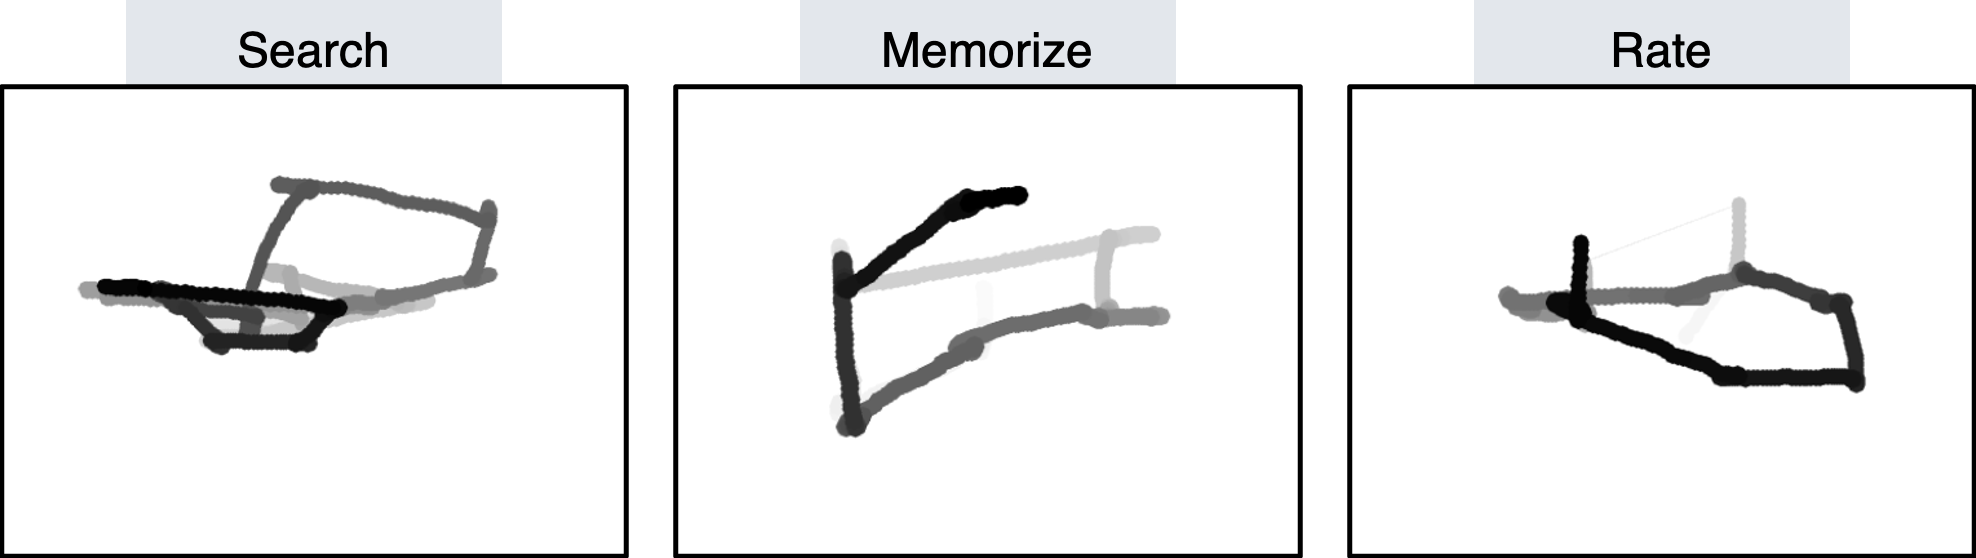
\includegraphics{figures/cond_imgs.png}
\caption{\label{fig:ave-condition}Each trial was represented as an image. Each sample collected within the trial was plotted as a dot in the image. Pupil size was represented by the size of the dot. The time course of the eye movements was represented by the gradual darkening of the dot over time.}
\end{figure}

\subsubsection{Data Subsets.}

The full timeline dataset was structured into three columns representing the x- and y- coordinates, and pupil size for each data point collected in the first six seconds of each trial. To systematically assess the predictive value of each XYP (i.e., x-coordinates, y-coordinates, pupil size) component of the data, the timeline and image datasets were batched into subsets that excluded one of the components (i.e., XY\(\varnothing\), X\(\varnothing\)P, \(\varnothing\)YP), or contained only one of the components (i.e., X\(\varnothing\varnothing\), \(\varnothing\)Y\(\varnothing\), \(\varnothing\varnothing\)P). For the timeline datasets, this means that the columns to be excluded in each data subset were replaced with zeros. The data were replaced with zeros because removing the columns would change the structure of the data. The same systematic batching process was carried out for the image dataset. See Figure \ref{fig:ave-subset} for an example of each of these image data subsets.

\begin{figure}
\centering
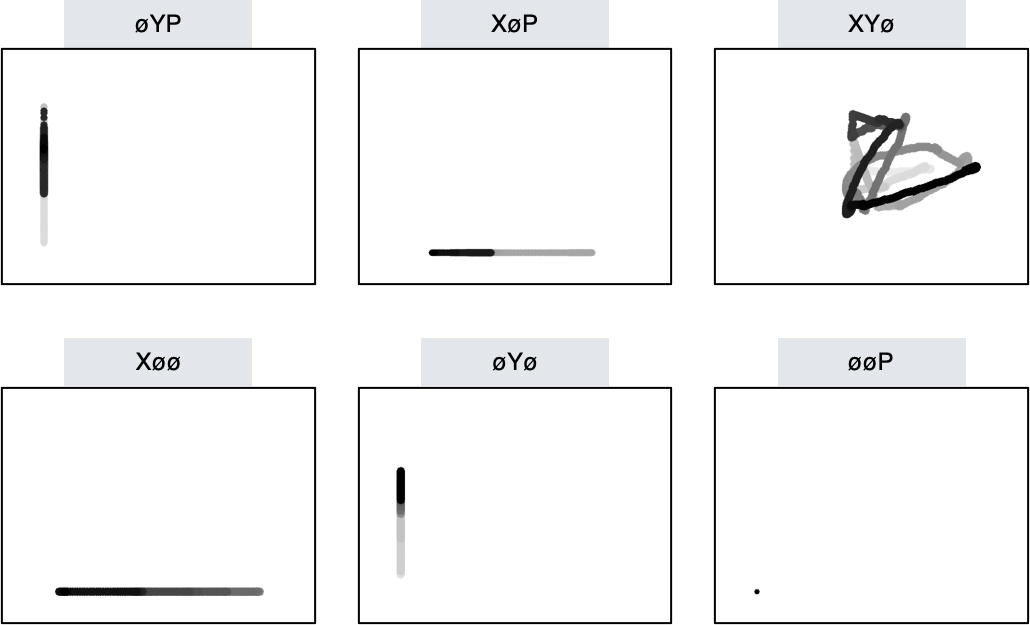
\includegraphics{figures/subset_imgs.png}
\caption{\label{fig:ave-subset}Plot images were used to represent each type of data subset. As with the trials in the full XYP dataset, the time course of the eye movements was represented by the shading of the dot. The first sample of each trial was white, and the last sample was black.}
\end{figure}

\subsection{Classification}

Deep CNN model architectures were implemented to classify the trials into Search, Memorize, or Rate categories. Because CNNs act as a digital filter sensitive to the number of features in the data, the differences in the structure of the timeline and image data formats necessitated separate CNN model architectures. The model architectures were developed with the intent of establishing a generalizable approach to classifying cognitive processes from eye movement data.

The development of these models was not guided by any formal theoretical assumptions regarding the patterns or features likely to be extracted by the classifier. Like many HCI models, the development of these models followed general intuitions concerned with building a model architecture capable of transforming the data inputs into an interpretable feature set that would not overfit the dataset. The models were developed using version 0.3b of the DeLINEATE toolbox, which operates over a Keras backend (\url{http://delineate.it}). Each training/test iteration randomly split the data so that 70\% of the trial data were allocated to training, 15\% of the trial data were allocated to validation, and 15\% of the trial data were allocated to testing. Training of the model was stopped when validation accuracy did not improve over the span of 100 epochs. Once the early stopping threshold was reached, the resulting model was tested on the held-out test data. This process was repeated 10 times for each model, resulting in 10 classification accuracy scores for each model. The average of the resulting accuracy scores were the subject of comparisons against chance and other datasets or data subsets.

The models were developed and tested on the Exploratory dataset. Model hyperparameters were adjusted until the classification accuracies appeared to peak. The model architecture with the highest classification accuracy on the Exploratory dataset was trained, validated, and tested independently on the Confirmatory dataset. This means that the model that was used to analyze the Confirmatory dataset was not trained on the Exploratory dataset. The model architectures used for the timeline and plot image datasets are shown in Figure \ref{fig:models}.

\begin{figure}
\centering
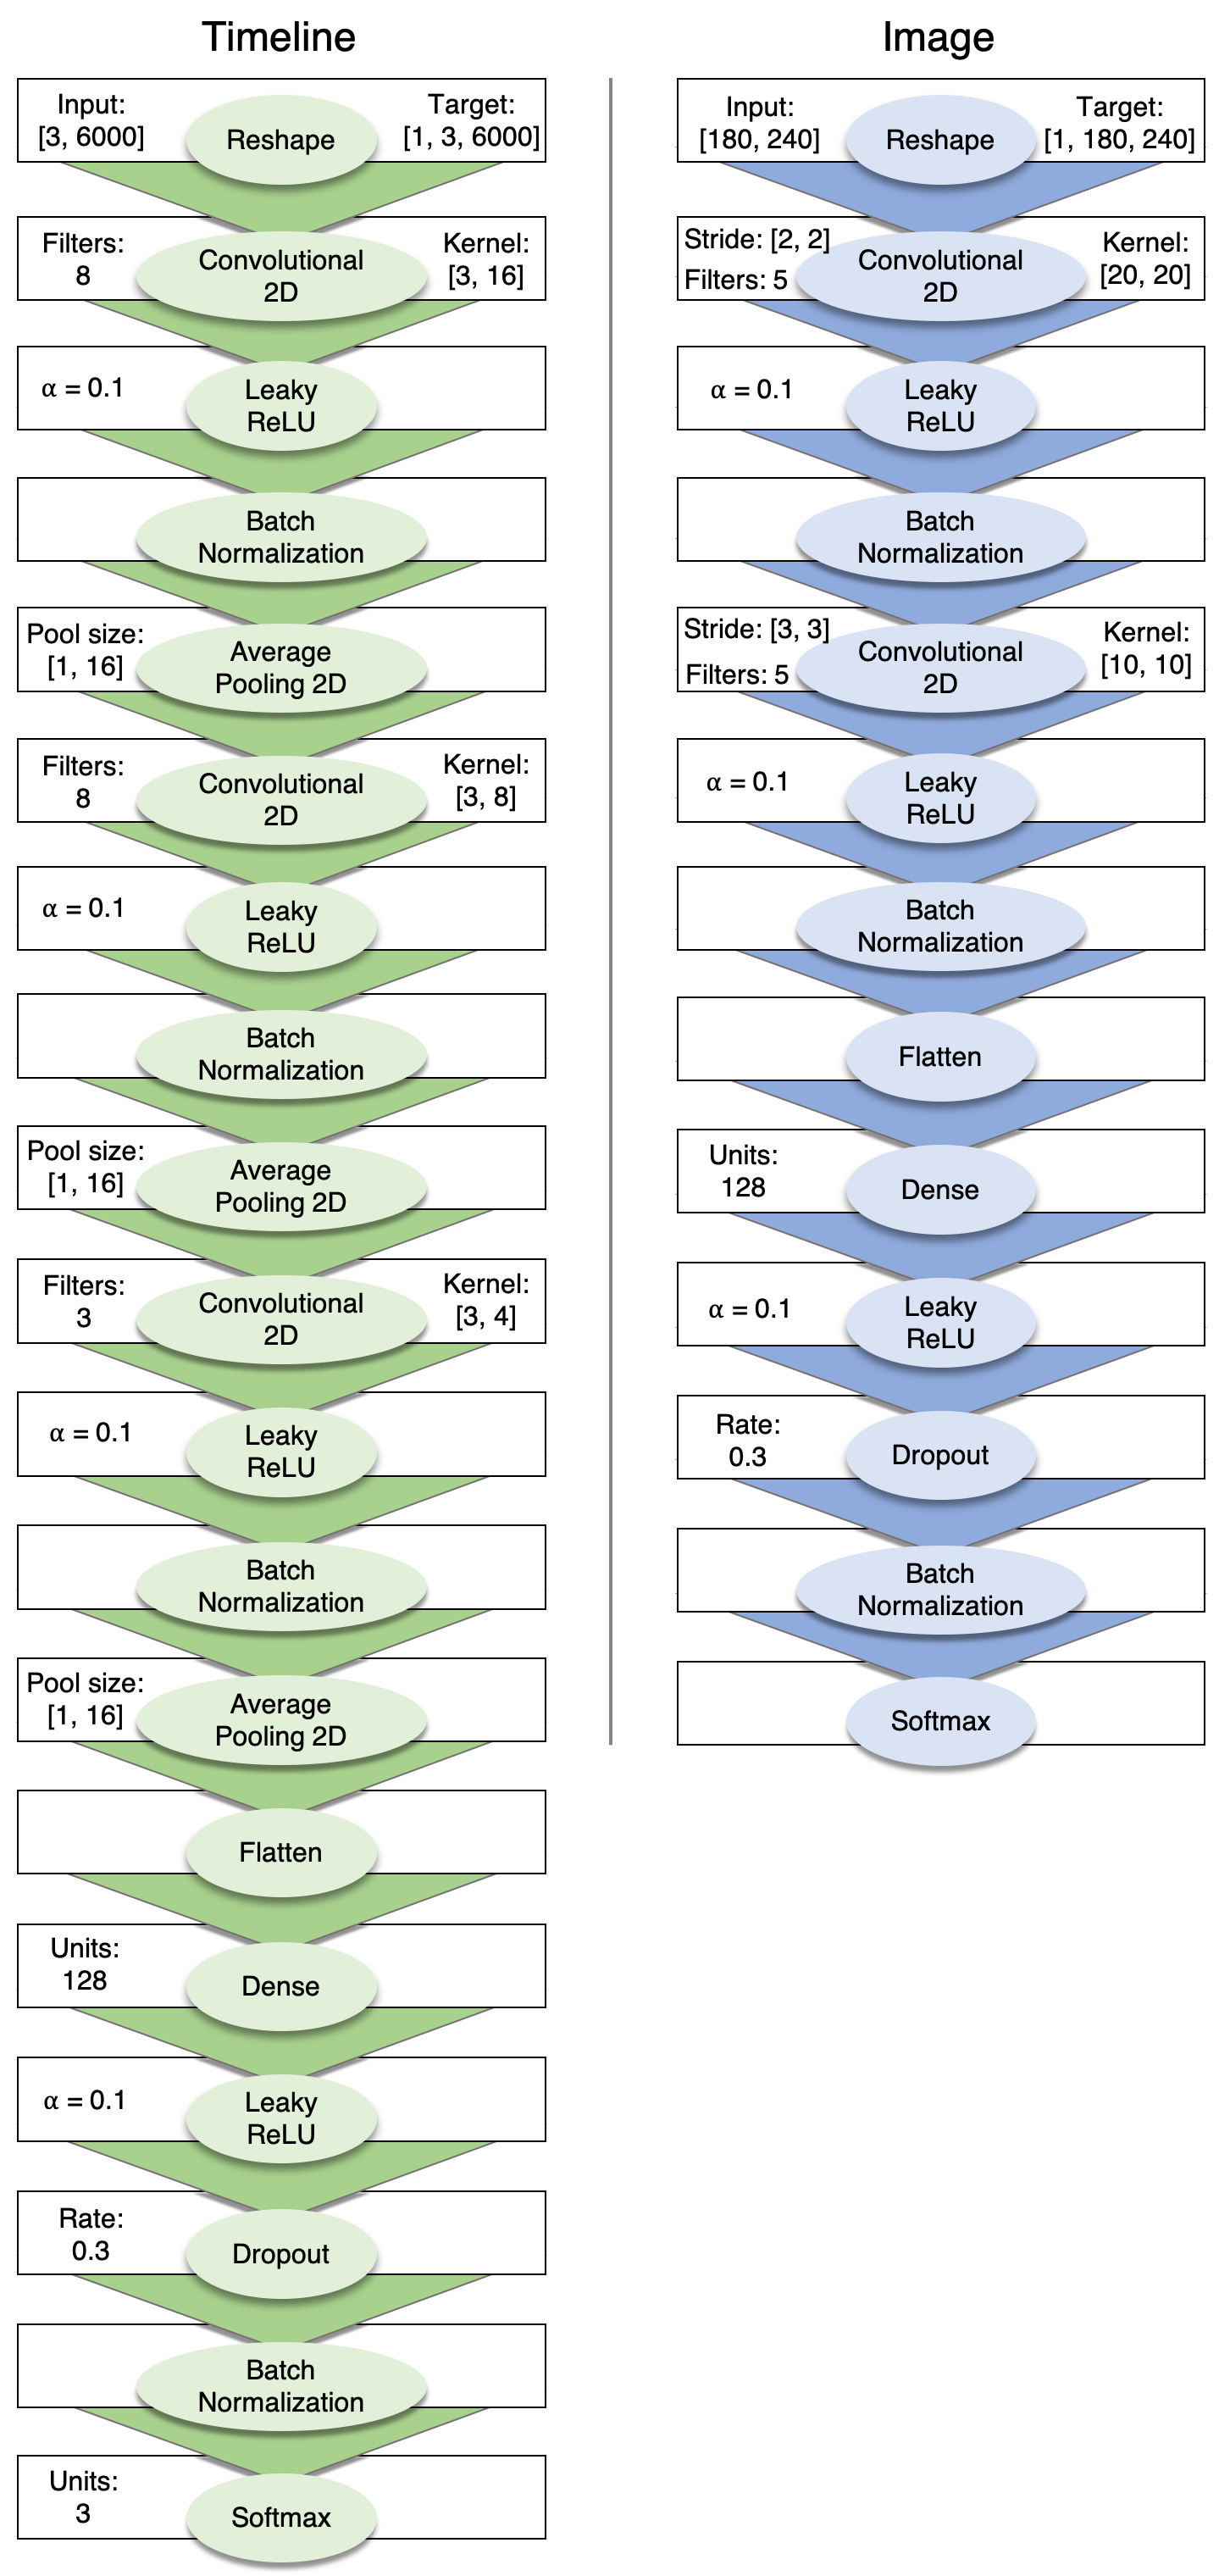
\includegraphics{figures/models.png}
\caption{\label{fig:models}Two different model architectures were used to classify the timeline and image data. Both models were compiled using a categorical crossentropy loss function, and optimized with the Adam algorithm.}
\end{figure}

\subsection{Analysis}

Results for the CNN architecture that resulted in the highest accuracy on the Exploratory dataset are reported below. For every dataset tested, a one-sample two-tailed \emph{t}-test was used to compare the CNN accuracies against chance (33\%). The Shapiro-Wilk test was used to assess the normality for each dataset. When normality was assumed, the mean accuracy for that dataset was compared against chance using Student's one-sample two-tailed \emph{t}-test. When normality could not be assumed, the median accuracy for that dataset was compared against chance using Wilcoxon's Signed Rank test.

To determine the relative value of the three components of the eye movement data, the data subsets were compared within the timeline and plot image data types. If classification accuracies were lower when the data were batched into subsets, the component that was removed was assumed to have some unique contribution that the model was using to inform classification decisions. To determine the relative value of the contribution from each component, the accuracies from each subset with one component of the data removed were compared to the accuracies for the full dataset (XYP) using a one-way between-subjects Analysis of Variance (ANOVA). To further evaluate the decodability of each component independently, the accuracies from each subset containing only one component of the eye movement data were compared within a separate one-way between-subjects ANOVA. All post-hoc comparisons were corrected using Tukey's HSD.

\section{Results}
\subsection{Timeline Data Classification}
\subsubsection{Exploratory.}

Classification accuracies for the XYP timeline dataset were well above chance (chance = 33\%; \emph{M} = .526, \emph{SD} = .018; \emph{t}\(_{(9)}\) = 34.565, \emph{p} \textless{} .001). Accuracies for classifications of the batched data subsets were all better than chance (see Figure \ref{fig:timeline-parcellation-chance}). As shown in the confusion matrices displayed in Figure \ref{fig:timeline-conf-matrices}, the data subsets with lower overall classification accuracies almost always classified the Memorize condition at or below chance levels of accuracy. Misclassifications of the Memorize condition were split relatively evenly between the Search and Rate conditions.

\begin{figure}
\centering
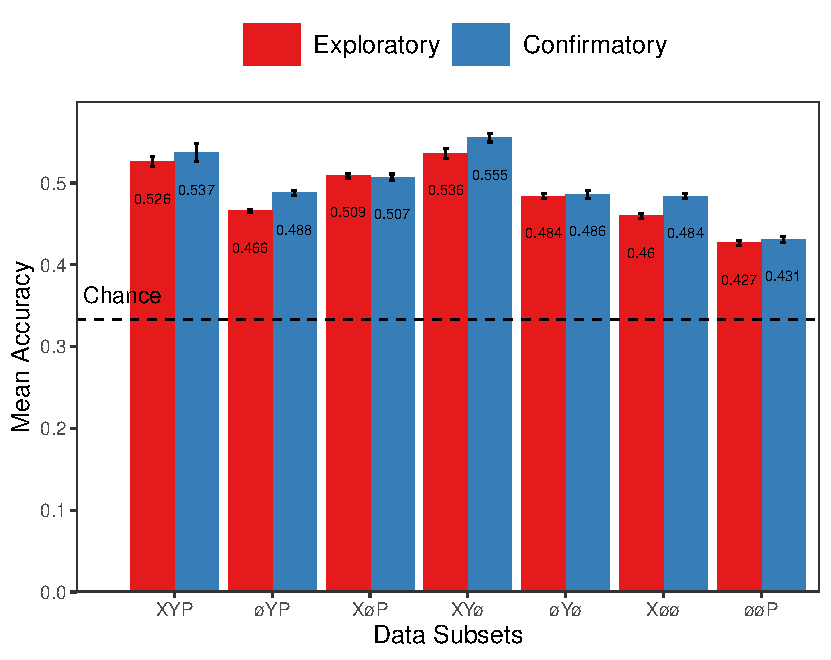
\includegraphics{results/r_code/timeline_subset_chance.pdf}
\caption{\label{fig:timeline-parcellation-chance}The graph represents the average accuracy reported for each subset of the timeline data. All of the data subsets were decoded at levels better than chance (33\%). Each subset is labeled with the mean accuracy. The error bars represent standard errors.}
\end{figure}

\begin{figure}
\centering
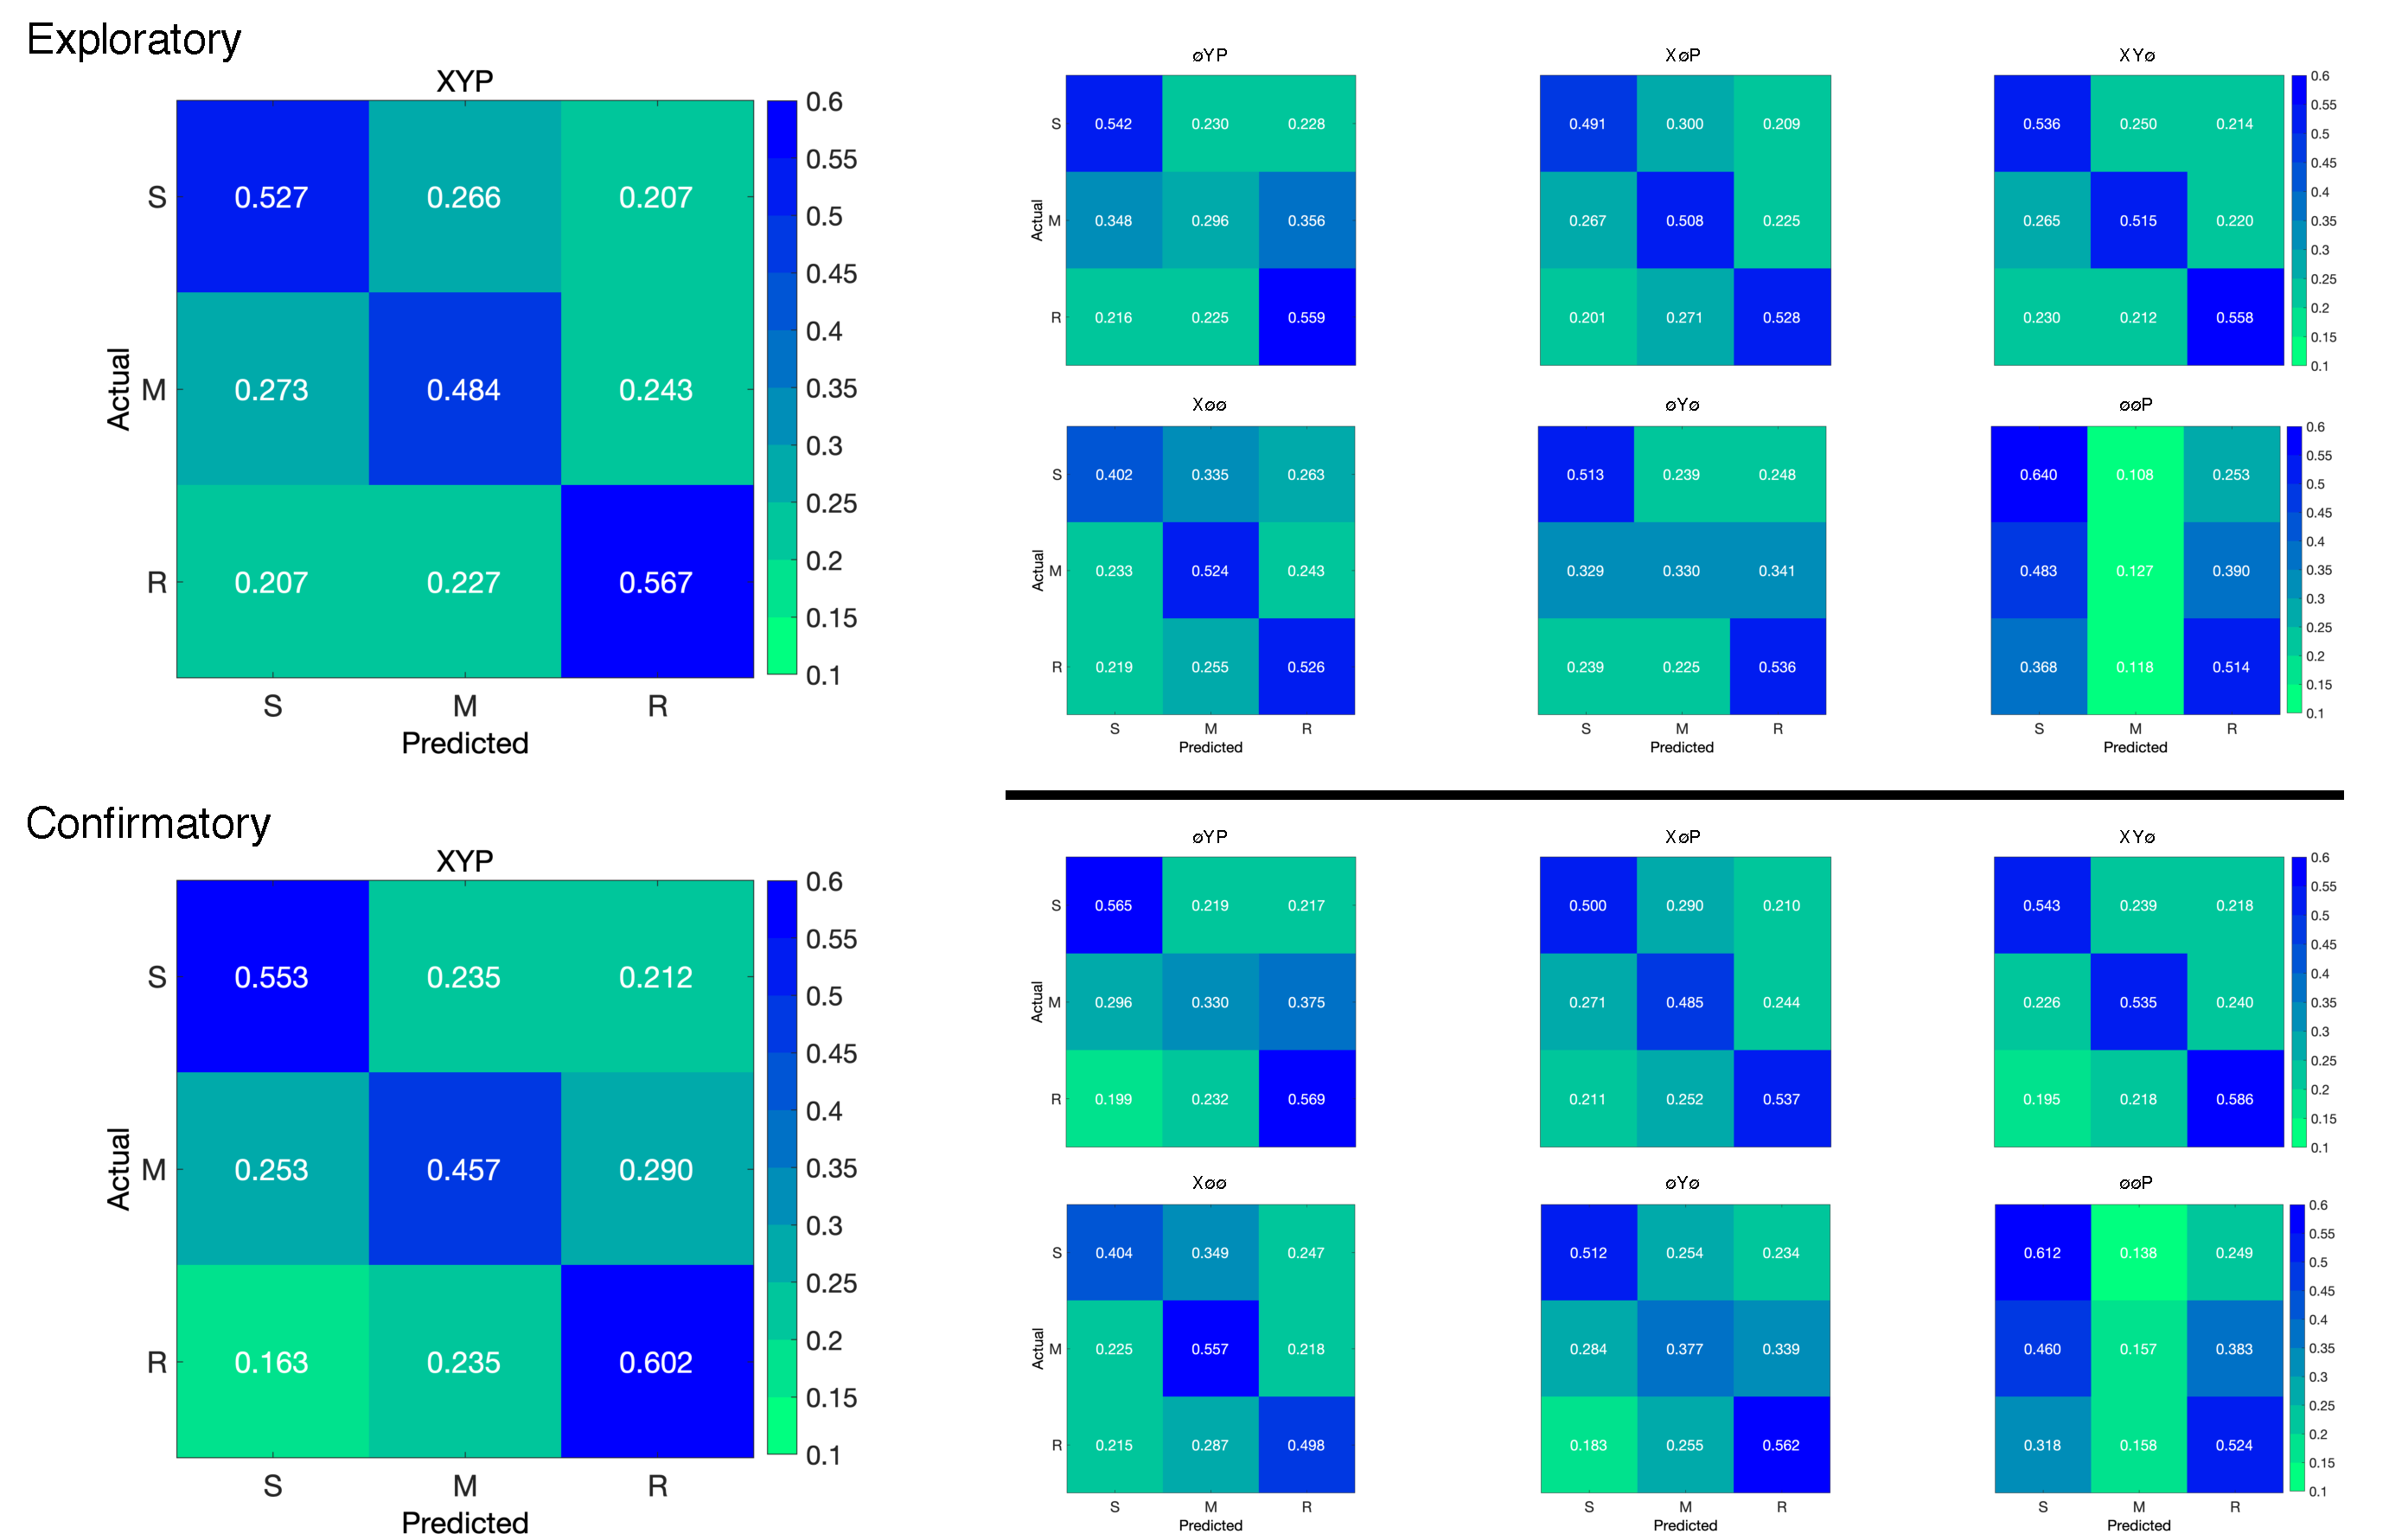
\includegraphics{figures/timeline_conf_matrices.pdf}
\caption{\label{fig:timeline-conf-matrices}The confusion matrices represent the average classification accuracies for each condition of the timeline data (S = Search, M = Memorize, R = Rate). The vertical axis of the confusion matrices represents the actual condition for trial. The horizontle axis of the confusion matrices represents the condition that was predicted by the model.}
\end{figure}

There was a difference in classification accuracy for the XYP dataset and the subsets that had the pupil size, x-coordinate, and y-coordinate data systematically removed (\emph{F}\(_{(3, 36)}\) = 47.471, \emph{p} \textless{} .001, \textit{$\eta$}\(^{2}\) = 0.798). Post-hoc comparisons against the XYP dataset showed that classification accuracies were not affected by the removal of pupil size or y-coordinate data (see Table \ref{tab:timeline-parcellation-comparisons}). The null effect present when pupil size was removed suggests that the pupil size data were not contributing unique information that was not otherwise provided by the x- and y-coordinates. A strict significance threshold of \(\alpha\) = .05 implies the same conclusion for the y-coordinate data, but the relatively low degrees of freedom (\emph{df} = 18) and the borderline observed \emph{p}-value (\emph{p} = .056) afford the possibility that there exists a small effect. However, classification for the \(\varnothing\)YP subset was significantly lower than the XYP dataset, showing that the x-coordinate data were uniquely informative to the classification.

\begin{table}[!h]
    \centering
    \caption{Timeline Subset Comparisons}
    \label{tab:timeline-parcellation-comparisons}
    \begin{tabular}{l c c c c}
         & \multicolumn{2}{c}{Exploratory} & \multicolumn{2}{c}{Confirmatory} \\
        \hline
        Comparison & \textit{t} & \multicolumn{1}{c|}{\textit{p}} & \textit{t} & \textit{p} \\
        \hline
        XYP vs. $\varnothing$YP & 9.420 & \multicolumn{1}{c|}{< .001} & 5.210 & < .001 \\
        XYP vs. X$\varnothing$P & 2.645 & \multicolumn{1}{c|}{.056} & 3.165 & .016 \\
        XYP vs. XY$\varnothing$ & 1.635 & \multicolumn{1}{c|}{.372} & 1.805 & .288 \\
        X$\varnothing\varnothing$ vs. $\varnothing$Y$\varnothing$ & 5.187 & \multicolumn{1}{c|}{< .001} & 0.495 & .874 \\
        X$\varnothing\varnothing$ vs. $\varnothing\varnothing$P & 12.213 & \multicolumn{1}{c|}{< .001} & 10.178 & < .001 \\
        $\varnothing$Y$\varnothing$ vs. $\varnothing\varnothing$P & 7.026 & \multicolumn{1}{c|}{< .001} & 9.683 & < .001 \\
        \hline
    \end{tabular}
\end{table}

There was also a difference in classification accuracies for the X\(\varnothing\varnothing\), \(\varnothing\)Y\(\varnothing\), and \(\varnothing\varnothing\)P subsets (\emph{F}\(_{(2, 27)}\) = 75.145, \emph{p} \textless{} .001, \textit{$\eta$}\(^{2}\) = 0.848). Post-hoc comparisons showed that classification accuracy for the \(\varnothing\varnothing\)P subset was lower than the X\(\varnothing\varnothing\) and \(\varnothing\)Y\(\varnothing\) subsets. Classification accuracy for the X\(\varnothing\varnothing\) subset was higher than the \(\varnothing\)Y\(\varnothing\) subset. Altogether, these findings suggest that pupil size data was the least uniquely informative to classification decisions, while the x-coordinate data was the most uniquely informative.

\subsubsection{Confirmatory.}

Classification accuracies for the Confirmatory XYP timeline dataset were well above chance (\emph{M} = .537, \emph{SD} = 0.036, \emph{t}\(_{(9)}\) = 17.849, \emph{p} \textless{} .001). Classification accuracies for the data subsets were also better than chance (see Figure \ref{fig:timeline-parcellation-chance}). Overall, there was high similarity in the pattern of results for the Exploratory and Confirmatory datasets (see Figure \ref{fig:timeline-parcellation-chance}). Furthermore, the general trend showing that pupil size was the least informative eye tracking data component was replicated in the Confirmatory dataset (see Table \ref{tab:timeline-parcellation-comparisons}). Also in concordance with the Exploratory timeline dataset, the confusion matrices for these data revealed that the Memorize task was mis-classified more often than the Search and Rate tasks (see Figure \ref{fig:timeline-conf-matrices}).

To test the generalizability of the model to other eye tracking data, classification accuracies for the XYP Exploratory and Confirmatory timeline datasets were compared. The Shapiro-Wilk test for normality indicated that the Exploratory (\emph{W} = 0.937, \emph{p} = .524) and Confirmatory (\emph{W} = 0.884, \emph{p} = .145) datasets were normally distributed, but Levene's test indicated that the variances were not equal, \emph{F}\(_{(1, 18)}\) = 8.783, \emph{p} = .008. Welch's unequal variances \emph{t}-test did not show a difference between the two datasets, \emph{t}\(_{(13.045)}\) = 0.907, \emph{p} = .381, Cohen's \emph{d} = 0.406. These findings indicate that the deep learning model decoded the Exploratory and Confirmatory timeline datasets equally well, but the Confirmatory dataset classifications were less consistent across training/test iterations (as indicated by the increase in standard deviation).

\subsection{Plot Image Classification}
\subsubsection{Exploratory.}

Classification accuracies for the XYP plot image data were better than chance (\emph{M} = .436, \emph{SD} = .020, \emph{p} \textless{} .001), but were less accurate than the classifications for the XYP Exploratory timeline data (\emph{t}\(_{(18)}\) = 10.813, \emph{p} \textless{} .001). Accuracies for the classifications for all subsets of the plot image data except the \(\varnothing\varnothing\)P subset were better than chance (see Figure \ref{fig:img-parcellation-chance}). Following the pattern expressed by the timeline dataset, the confusion matrices showed that the Memorize condition was misclassified more often than the other conditions, and appeared to be evenly mis-identified as a Search or Rate condition (see Figure \ref{fig:img-conf-matrices}).

\begin{figure}
\centering
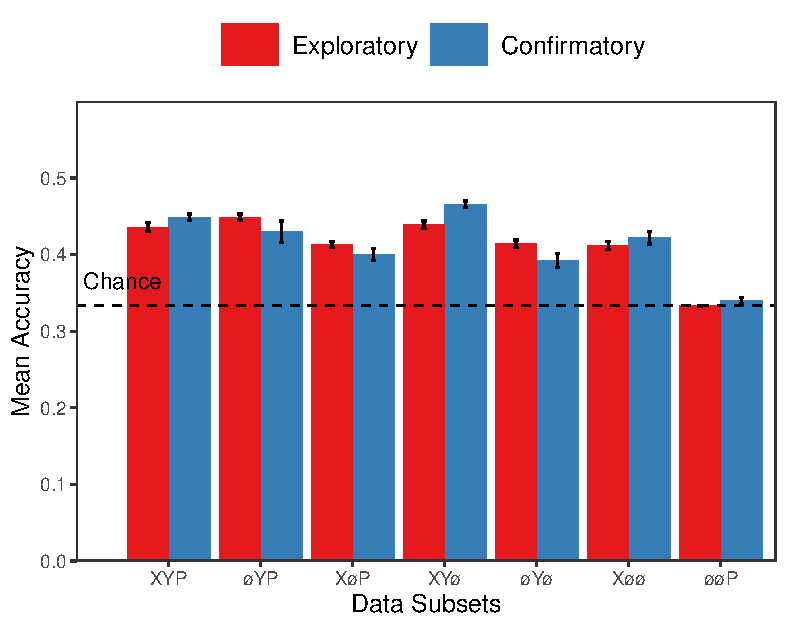
\includegraphics{results/r_code/img_subset_chance.pdf}
\caption{\label{fig:img-parcellation-chance}The graph represents the average accuracy reported for each subset of the image data. All of the data subsets except for the Exploratory \(\varnothing\varnothing\)P dataset were decoded at levels better than chance (33\%). Each subset is labeled with the mean accuracy. The error bars represent standard errors.}
\end{figure}

\begin{figure}
\centering
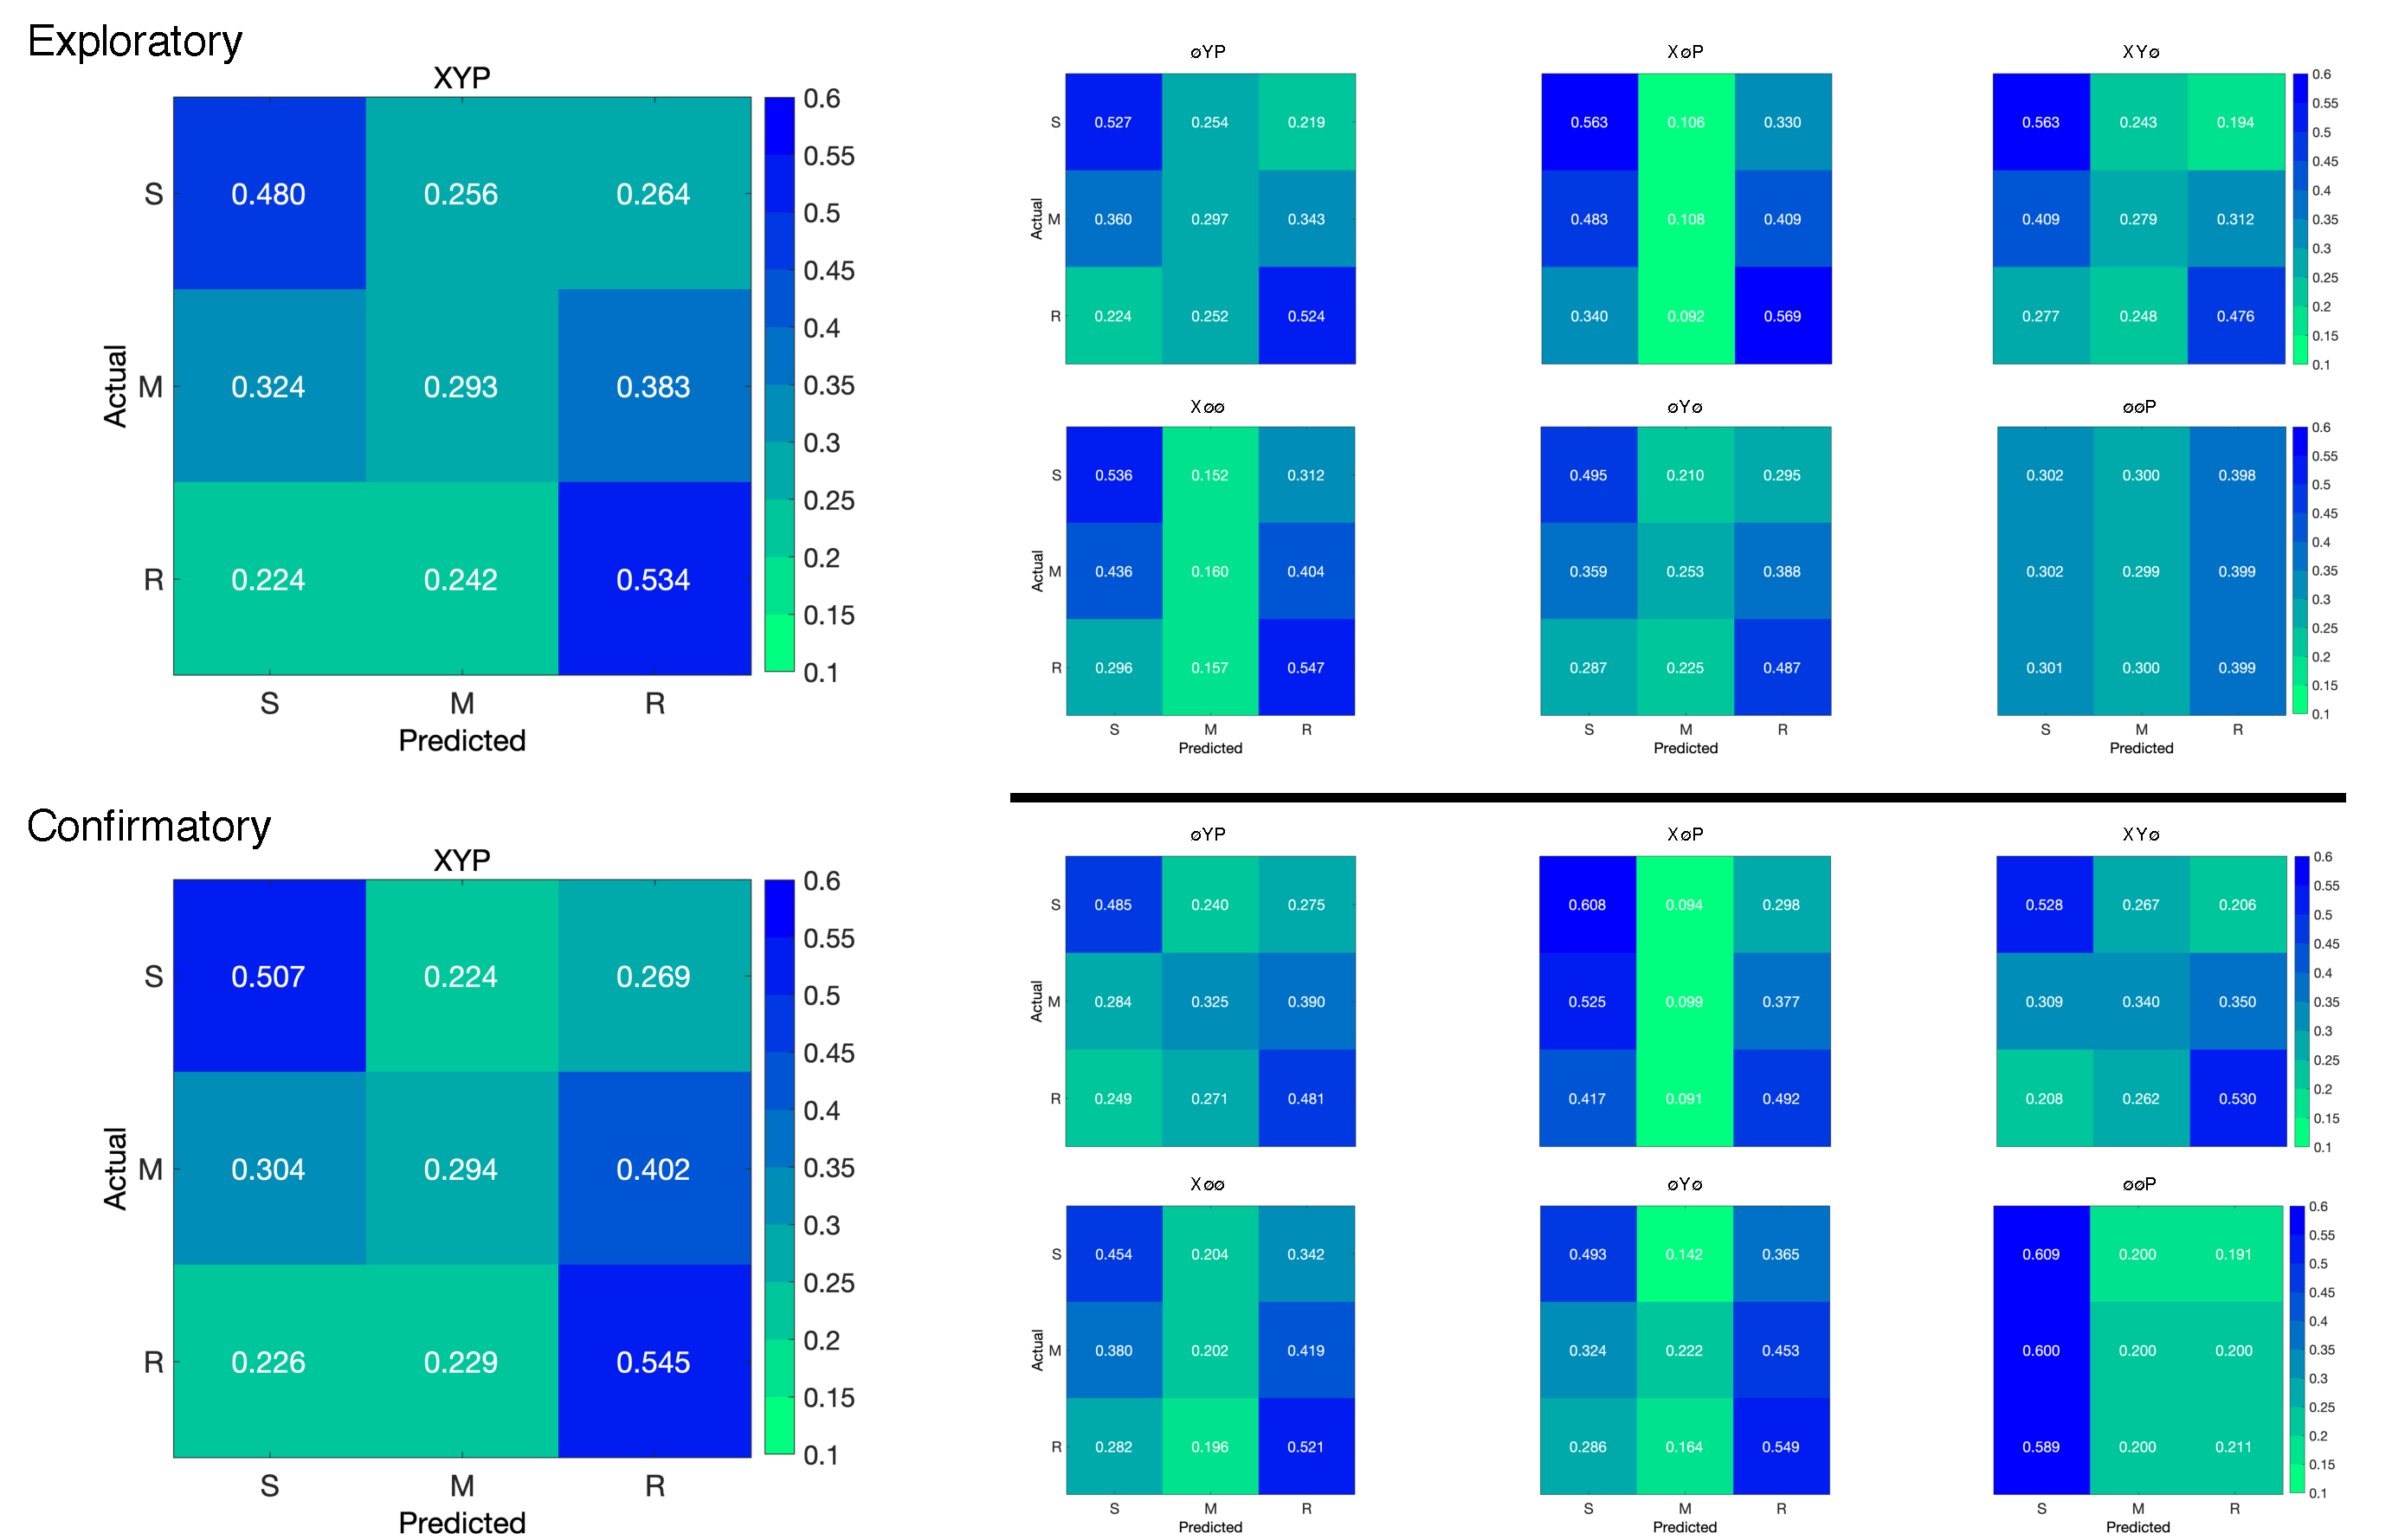
\includegraphics{figures/img_conf_matrices.pdf}
\caption{\label{fig:img-conf-matrices}The confusion matrices represent the average classification accuracies for each condition of the image data (S = Search, M = Memorize, R = Rate). The vertical axis of the confusion matrices represents the actual condition for the trial. The horizontle axis of the confusion matrices represents the condition that was predicted by the model.}
\end{figure}

There was a difference in classification accuracy between the XYP dataset and the data subsets (\emph{F}\(_{(4, 45)}\) = 7.093, \emph{p} \textless{} .001, \textit{$\eta$}\(^{2}\) = .387). Post-hoc comparisons showed that compared to the XYP dataset, there was no effect of removing pupil size or the x-coordinates, but classification accuracy was worse when the y-coordinates were removed (see Table \ref{tab:image-parcellation-comparisons}).

\begin{table}[!h]
    \centering
    \caption{Image Subset Comparisons}
    \label{tab:image-parcellation-comparisons}
    \begin{tabular}{l c c c c}
         & \multicolumn{2}{c}{Exploratory} & \multicolumn{2}{c}{Confirmatory} \\
        \hline
        Comparison & \textit{t} & \multicolumn{1}{c|}{\textit{p}} & \textit{t} & \textit{p} \\
        \hline
        XYP vs. $\varnothing$YP & 1.792 & \multicolumn{1}{c|}{.391} & 1.623 & .491 \\
        XYP vs. X$\varnothing$P & 2.939 & \multicolumn{1}{c|}{.039} & 4.375 & < .001 \\
        XYP vs. XY$\varnothing$ & 0.474 & \multicolumn{1}{c|}{.989} & 1.557 & .532 \\
        X$\varnothing\varnothing$ vs. $\varnothing$Y$\varnothing$ & 0.423 & \multicolumn{1}{c|}{.906} & 2.807 & .204 \\
        X$\varnothing\varnothing$ vs. $\varnothing\varnothing$P & 13.569 & \multicolumn{1}{c|}{< .001} & 5.070 & < .001 \\
        $\varnothing$Y$\varnothing$ vs. $\varnothing\varnothing$P & 13.235 & \multicolumn{1}{c|}{< .001} & 7.877 & < .001 \\
        \hline
    \end{tabular}
\end{table}

There was also a difference in classification accuracies between the X\(\varnothing\varnothing\), \(\varnothing\)Y\(\varnothing\), and \(\varnothing\varnothing\)P subsets (Levene's test: \emph{F}\(_{(2, 27)}\) = 3.815, \emph{p} = .035; Welch correction for lack of homogeneity of variances: \emph{F}\(_{(2, 17.993)}\) = 228.137, \emph{p} \textless{} .001, \textit{$\eta$}\(^{2}\) = .899). Post-hoc comparisons showed that there was no difference in classification accuracies for the X\(\varnothing\varnothing\) and \(\varnothing\)Y\(\varnothing\) subsets, but classification for the \(\varnothing\varnothing\)P subset were less accurate than the X\(\varnothing\varnothing\) and \(\varnothing\)Y\(\varnothing\) subsets.

\subsubsection{Confirmatory.}

Classification accuracies for the XYP confirmatory image dataset were well above chance (\emph{M} = .449, \emph{SD} = 0.012, \emph{t}\(_{(9)}\) = 31.061, \emph{p} \textless{} .001), but were less accurate than the classifications of the confirmatory timeline dataset (\emph{t}\(_{(18)}\) = 11.167 \emph{p} \textless{} .001). Accuracies for classifications of the data subsets were also all better than chance (see Figure \ref{fig:img-parcellation-chance}). The confusion matrices followed the pattern showing that the Memorize condition was confused most often, and was relatively evenly mis-identified as a Search or Rate trial (see Figure \ref{fig:img-conf-matrices}). As with the timeline data, the general trend showing that pupil size data was the least informative to the model was replicated in the Confirmatory dataset (see Table \ref{tab:image-parcellation-comparisons}).

To test the generalizability of the model, the classification accuracies for the XYP Exploratory and Confirmatory plot image datasets were compared. The independent samples \emph{t}-test showed that the deep learning model did equally well at classifying the Exploratory and Confirmatory plot image datasets, \emph{t}\(_{(18)}\) = 1.777, \emph{p} = .092, Cohen's \emph{d} = 0.795.

\section{Discussion}

The present study aimed to produce a practical and reliable example of a black box solution to the inverse Yarbus problem. To implement this solution, we classified raw timeline and minimally processed plot image data using a CNN model architecture. To our knowledge, this study was the first to provide a solution to determining mental state from eye movement data using each of the following: (1) Non-aggregated eye tracking data (i.e., raw x-coordinates, y-coordinates, pupil size), (2) timeline and image data formats (see Figure \ref{fig:ave-subset}), and (3) a black box CNN architecture. This study probed the relative predictive value of the x-coordinate, y-coordinate, and pupil size components of the eye movement data using a CNN. The CNN was able to decode the timeline and plot image data better than chance, although only the timeline datasets were decoded with accuracies comparable to other state-of-the-art approaches. Datasets with lower classification accuracies were not able to differentiate the cognitive processes underlying the Memorize task from the cognitive processes underlying the Search and Rate tasks. Decoding subsets of the data revealed that pupil size was the least uniquely informative component of the eye movement data. This pattern of findings was consistent between the Exploratory and Confirmatory datasets.

Although several aggregate eye movement features have been tested as task predictors, to our knowledge, no other study has assessed the predictive value of the data format (viz., data in the format of a plot image). Our results suggest that although CNNs are robust image classifiers, eye movement data is decoded in the standard timeline format more effectively than in image format. This may be because the image data format contains less decodable information than the timeline format. Over the span of the trial (six seconds), the eye movements occasionally overlapped. When there was an overlap in the image data format, the more recent data points overwrote the older data points. This resulted in some information loss that did not occur when the data were represented in the raw timeline format. Despite this loss of information, the plot image format was still decoded with better than chance accuracy. To further examine the viability of classifying task from eye movement image datasets, future research might consider representing the data in different forms such as 3-dimensional data formats, or more complex color combinations capable of representing overlapping data points.

When considering the superior performance of the timeline data (vs., plot image data), we must also consider the differences in the model architectures. Because the structures of the timeline and plot image data formats were different, the models decoding those data structures also needed to be different. Both models were optimized individually on the Exploratory dataset before being tested on the Confirmatory dataset. For both timeline and plot image formats, there was good replicability between the Exploratory and Confirmatory datasets, demonstrating that these architectures performed similarly from experiment to experiment. An appropriately tuned CNN should be capable of learning any arbitrary function, but given that the upper bound for decodability of these datasets is unknown, there is the possibility that a model architecture exists that is capable of classifying the plot image data format more accurately than the model used to classify the timeline data. Despite this possibility, the convergence of these findings with other studies (see Table \ref{tab:previous-studies}) suggests that the results of this study are approaching a ceiling for the potential to solve the inverse Yarbus problem with eye movement data. Although the true capacity to predict mental state from eye movement data is unknown, standardizing datasets in the future could provide a point for comparison that can more effectively indicate which methods are most effective at solving the inverse Yarbus problem.

In the current study, the Memorize condition was most classified less accurately than the Search and Rate conditions, especially for the datasets with lower overall accuracy. This suggests that the eye movements associated with the Memorize task were potentially lacking unique or informative features to decode. This means that eye movements associated with the Memorize condition were interpreted as noise, or were sharing features of underlying cognitive processes that were represented in the eye movements associated with the Search and Rate tasks. Previous research (e.g., Król \& Król, 2018) has attributed the inability to differentiate one condition from the others to the overlapping of sub-features in the eye movements between two tasks that are too subtle to be represented in the eye movement data.

To more clearly understand how the different tasks influenced the decodability of the eye movement data, additional analyses were conducted on the Exploratory and Confirmatory timeline datasets (see Appendix). These analyses showed that classification accuracy improved when the Memorize condition was removed. A closer look at these results showed that when the Memorize condition was included in the subset, classification accuracies of the Search and Rate conditions was lower. The analyses were complemented with a re-calculation of the accuracies from the primary analysis to account for a 50\% threshold of chance performance. Altogether, these results could indicate that the eye movement features underlying the Memorize condition are shared with the Search and Rate conditions, or that the Memorize condition is contributing a substantial amount of noise. Given the findings of these supplementary analyses, we belive that the Memorize trials were more often mis-classified than the other trials due to an increased prevalence of noise in the eye movement data for the Memorize trials.

When determining the relative contributions of the the eye movement features used in this study (x-coordinates, y-coordinates, pupil size), the pupil size data was consistently the least uniquely informative. When pupil size was removed from the Exploratory and Confirmatory timeline and plot image datasets, classification accuracy remained stable (vs., XYP dataset). Furthermore, classification of the \(\varnothing\varnothing\)P subset was the lowest of all of the data subsets, and in one instance, was no better than chance. Although these findings indicate that, in this case, pupil size was a relatively uninformative component of the eye movement data, previous research has associated changes in pupil size as indicators of working memory load (Kahneman \& Beatty, 1966; Karatekin, Couperus, \& Marcus, 2004), arousal (Wang et al., 2018), and cognitive effort (Porter, Troscianko, \& Gilchrist, 2007). The results of the current study indicate that the changes in pupil size associated with these underlying processes are not useful in delineating the tasks being classified (i.e., Search, Memorize, Rate), potentially because these tasks do not evoke a reliable pattern of changes in pupil size.

The findings from the current study support the notion that black box CNNs are a viable approach to determining task from eye movement data. In a recent review, Lukander et al. (2017) expressed concern regarding the lack of generalizability of black box approaches when decoding eye movement data. Overall, the current study showed a consistent pattern of results for the XYP timeline and image datasets, but some minor inconsistencies in the pattern of results for the x- and y- coordinate subset comparisons. These inconsistencies may be a product of overlap in the cognitive processes underlying the three tasks. When the data are batched into subsets, at least one dimension (i.e., x-coordinates, y-coordinates, or pupil size) is removed, leading to a potential loss of information. When the data provide fewer meaningful distinctions, finer-grained inferences are necessary for the tasks to be distinguishable. As shown by Coco and Keller (2014), eye movement data can be more effectively decoded when the cognitive processes underlying the tasks are explicitly differentiable. While the cognitive processes distinguishing memorizing, searching, or rating an image are intuitively different, the eye movements elicited from these cognitive processes are not easily differentiated. To correct for potential mismatches between the distinctive task-diagnostic features in the data and the level of distinctiveness required to classify the tasks, future research could more definitively conceptualize the cognitive processes underlying the task-at-hand.

Classifying mental state from eye movement data is often carried out in an effort to advance technology to improve educational outcomes, strengthen the independence of physically and mentally handicapped individuals, or improve HCI's (Koochaki \& Najafizadeh, 2018). Given the previous questions raised regarding the reliability and generalizability of black-box CNN classification, the current study first tested models on an exploratory dataset, then confirmed the outcome using a second independent dataset. Overall, the findings of this study indicate that this black-box approach is capable of producing a stable and generalizable outcome. Future studies that incorporate stimulus features might have the potential to surpass current state-of-the-art classification. According to Bulling, Weichel, and Gellersen (2013), incorporating stimulus feature information into the dataset may provide improve accuracy relative to decoding gaze location data and pupil size. Alternatively, Borji and Itti (2014) suggested that accounting for salient features in the the stimulus might leave little to no room for theoretically defined classifiers to consider mental state. Future research should examine the potential for the inclusion of stimulus feature information in addition to the eye movement data to boost black-box CNN classification accuracy of image data beyond that of timeline data.

\newpage

\hypertarget{references}{%
\section{References}\label{references}}

\begingroup
\setlength{\parindent}{-0.5in}
\setlength{\leftskip}{0.5in}

\hypertarget{refs}{}
\leavevmode\hypertarget{ref-boisvertPredictingTaskEye2016}{}%
Boisvert, J. F. G., \& Bruce, N. D. B. (2016). Predicting task from eye movements: On the importance of spatial distribution, dynamics, and image features. \emph{Neurocomputing}, \emph{207}, 653--668. \url{https://doi.org/10.1016/j.neucom.2016.05.047}

\leavevmode\hypertarget{ref-borjiDefendingYarbusEye2014a}{}%
Borji, A., \& Itti, L. (2014). Defending Yarbus: Eye movements reveal observers' task. \emph{Journal of Vision}, \emph{14}(3), 29--29. \url{https://doi.org/10.1167/14.3.29}

\leavevmode\hypertarget{ref-bullingEyeContextRecognitionHighlevel2013}{}%
Bulling, A., Weichel, C., \& Gellersen, H. (2013). EyeContext: Recognition of high-level contextual cues from human visual behaviour. In \emph{Proceedings of the SIGCHI Conference on Human Factors in Computing Systems - CHI '13} (p. 305). Paris, France: ACM Press. \url{https://doi.org/10.1145/2470654.2470697}

\leavevmode\hypertarget{ref-castelhanoViewingTaskInfluences2009}{}%
Castelhano, M. S., Mack, M. L., \& Henderson, J. M. (2009). Viewing task influences eye movement control during active scene perception. \emph{Journal of Vision}, \emph{9}(3), 6--6. \url{https://doi.org/10.1167/9.3.6}

\leavevmode\hypertarget{ref-cocoClassificationVisualLinguistic2014}{}%
Coco, M. I., \& Keller, F. (2014). Classification of visual and linguistic tasks using eye-movement features. \emph{Journal of Vision}, \emph{14}(3), 11--11. \url{https://doi.org/10.1167/14.3.11}

\leavevmode\hypertarget{ref-deangelusTopdownControlEye2009}{}%
DeAngelus, M., \& Pelz, J. B. (2009). Top-down control of eye movements: Yarbus revisited. \emph{Visual Cognition}, \emph{17}(6-7), 790--811. \url{https://doi.org/10.1080/13506280902793843}

\leavevmode\hypertarget{ref-greeneReconsideringYarbusFailure2012a}{}%
Greene, M. R., Liu, T., \& Wolfe, J. M. (2012). Reconsidering Yarbus: A failure to predict observers' task from eye movement patterns. \emph{Vision Res}, \emph{62}, 1--8. \url{https://doi.org/10.1016/j.visres.2012.03.019}

\leavevmode\hypertarget{ref-haji-abolhassaniInverseYarbusProcess2014}{}%
Haji-Abolhassani, A., \& Clark, J. J. (2014). An inverse Yarbus process: Predicting observers' task from eye movement patterns. \emph{Vision Research}, \emph{103}, 127--142. \url{https://doi.org/10.1016/j.visres.2014.08.014}

\leavevmode\hypertarget{ref-hendersonPredictingCognitiveState2013a}{}%
Henderson, J. M., Shinkareva, S. V., Wang, J., Luke, S. G., \& Olejarczyk, J. (2013). Predicting Cognitive State from Eye Movements. \emph{PLoS ONE}, \emph{8}(5), e64937. \url{https://doi.org/10.1371/journal.pone.0064937}

\leavevmode\hypertarget{ref-kahnemanPupilDiameterLoad1966}{}%
Kahneman, D., \& Beatty, J. (1966). Pupil Diameter and Load on Memory. \emph{Science}, \emph{154}(3756), 1583--1585. Retrieved from \url{https://www.jstor.org/stable/1720478}

\leavevmode\hypertarget{ref-kananPredictingObserverTask2014}{}%
Kanan, C., Ray, N. A., Bseiso, D. N. F., Hsiao, J. H., \& Cottrell, G. W. (2014). Predicting an observer's task using multi-fixation pattern analysis. In \emph{Proceedings of the Symposium on Eye Tracking Research and Applications - ETRA '14} (pp. 287--290). Safety Harbor, Florida: ACM Press. \url{https://doi.org/10.1145/2578153.2578208}

\leavevmode\hypertarget{ref-karatekinAttentionAllocationDualtask2004}{}%
Karatekin, C., Couperus, J. W., \& Marcus, D. J. (2004). Attention allocation in the dual-task paradigm as measured through behavioral and psychophysiological responses. \emph{Psychophysiology}, \emph{41}(2), 175--185. \url{https://doi.org/10.1111/j.1469-8986.2004.00147.x}

\leavevmode\hypertarget{ref-koochakiPredictingIntentionEye2018}{}%
Koochaki, F., \& Najafizadeh, L. (2018). Predicting Intention Through Eye Gaze Patterns. In \emph{2018 IEEE Biomedical Circuits and Systems Conference (BioCAS)} (pp. 1--4). \url{https://doi.org/10.1109/BIOCAS.2018.8584665}

\leavevmode\hypertarget{ref-krolRightLookJob2018}{}%
Król, M. E., \& Król, M. (2018). The right look for the job: Decoding cognitive processes involved in the task from spatial eye-movement patterns. \emph{Psychological Research}. \url{https://doi.org/10.1007/s00426-018-0996-5}

\leavevmode\hypertarget{ref-lukanderInferringIntentAction2017}{}%
Lukander, K., Toivanen, M., \& Puolamäki, K. (2017). Inferring Intent and Action from Gaze in Naturalistic Behavior: A Review. \emph{International Journal of Mobile Human Computer Interaction}, \emph{9}(4), 41--57. \url{https://doi.org/10.4018/IJMHCI.2017100104}

\leavevmode\hypertarget{ref-macinnesjosephGenerativeModelCognitive2018}{}%
MacInnes, W., Joseph, Hunt, A. R., Clarke, A. D. F., \& Dodd, M. D. (2018). A Generative Model of Cognitive State from Task and Eye Movements. \emph{Cognitive Computation}, \emph{10}(5), 703--717. \url{https://doi.org/10.1007/s12559-018-9558-9}

\leavevmode\hypertarget{ref-millsExaminingInfluenceTask2011}{}%
Mills, M., Hollingworth, A., Van der Stigchel, S., Hoffman, L., \& Dodd, M. D. (2011). Examining the influence of task set on eye movements and fixations. \emph{Journal of Vision}, \emph{11}(8), 17--17. \url{https://doi.org/10.1167/11.8.17}

\leavevmode\hypertarget{ref-porterEffortVisualSearch2007}{}%
Porter, G., Troscianko, T., \& Gilchrist, I. D. (2007). Effort during visual search and counting: Insights from pupillometry. \emph{Quarterly Journal of Experimental Psychology (2006)}, \emph{60}(2), 211--229. \url{https://doi.org/10.1080/17470210600673818}

\leavevmode\hypertarget{ref-seeligerConvolutionalNeuralNetworkbased2018}{}%
Seeliger, K., Fritsche, M., Güçlü, U., Schoenmakers, S., Schoffelen, J.-M., Bosch, S. E., \& van Gerven, M. A. J. (2018). Convolutional neural network-based encoding and decoding of visual object recognition in space and time. \emph{NeuroImage}, \emph{180}, 253--266. \url{https://doi.org/10.1016/j.neuroimage.2017.07.018}

\leavevmode\hypertarget{ref-tatlerYarbusEyeMovements2010}{}%
Tatler, B. W., Wade, N. J., Kwan, H., Findlay, J. M., \& Velichkovsky, B. M. (2010). Yarbus, Eye Movements, and Vision. \emph{I-Perception}, \emph{1}(1), 7--27. \url{https://doi.org/10.1068/i0382}

\leavevmode\hypertarget{ref-wangArousalEffectsPupil2018}{}%
Wang, C.-A., Baird, T., Huang, J., Coutinho, J. D., Brien, D. C., \& Munoz, D. P. (2018). Arousal Effects on Pupil Size, Heart Rate, and Skin Conductance in an Emotional Face Task. \emph{Frontiers in Neurology}, \emph{9}. \url{https://doi.org/10.3389/fneur.2018.01029}

\leavevmode\hypertarget{ref-yarbusEyeMovementsVision1967}{}%
Yarbus, A. (1967). Eye Movements and Vision. Retrieved January 24, 2019, from \url{http://wexler.free.fr/library/files/yarbus\%20(1967)\%20eye\%20movements\%20and\%20vision.pdf}

\leavevmode\hypertarget{ref-zhouComparingInterpretabilityDeep2019}{}%
Zhou, B., Bau, D., Oliva, A., \& Torralba, A. (2019). Comparing the Interpretability of Deep Networks via Network Dissection. In W. Samek, G. Montavon, A. Vedaldi, L. K. Hansen, \& K.-R. Müller (Eds.), \emph{Explainable AI: Interpreting, Explaining and Visualizing Deep Learning} (pp. 243--252). Cham: Springer International Publishing. \url{https://doi.org/10.1007/978-3-030-28954-6_12}

\endgroup

\clearpage
\makeatletter
\efloat@restorefloats
\makeatother


\begin{appendix}
\hypertarget{supplementary-analysis}{%
\section{Supplementary Analysis}\label{supplementary-analysis}}

Additional analyses were conducted to clarify the effect of task on
classification accuracy. These supplementary analyses were not seen as
central to the current study, but could prove to be informative to
researchers attempting to replicate or extend these findings in the
future. The results from the primary analyses showed that classification
accuracies were the lowest for the Memorize condition, but these
findings did not indicate if the Memorize condition was adding noise to
the data, or was providing redundant information to the model. To
further understand why classification accuracy was lower for the
Memorize condition than it was for the Search or Rate condition, the
Exploratory and Confirmatory timeline datasets were systematically
batched into subsets with the Search (S), Memorize (M), or Rate (R)
condition removed (i.e., \(\varnothing\)MR, S\(\varnothing\)R,
SM\(\varnothing\)).

All of the data subsets analyzed in this supplementary analysis were
decoded with better than chance accuracy (see Figure
\ref{fig:supp-chance}). The same pattern of results was observed in both
the Exploratory and Confirmatory datasets. When the Memorize condition
was removed, classification accuracy improved (see Table
\ref{tab:supp-comparisons}). When the Rate condition was removed,
classification was the worst. When the Memorize condition was included,
the Memorize condition was more accurately predicted than the Search and
Rate conditions (see Figure \ref{fig:supp-conf-matrices}).

\begin{figure}
\centering
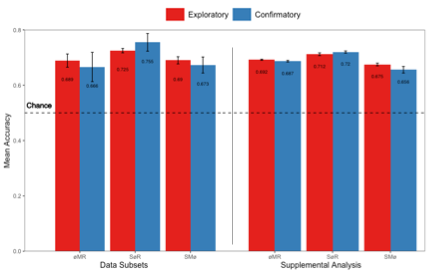
\includegraphics{supplementary_analysis/recalc_orig_accs/recalc_bar_graph.png}
\caption{\label{fig:supp-chance}The graph represents the average accuracy
reported for each subset of the Exploratory and Confirmatory timeline
data for the supplementary analysis and the re-calculated accuracies
from the primary analyses. All of the data subsets were decoded at
levels better than chance (50\%). The error bars represent standard
errors.}
\end{figure}

\begin{table}[!h]
\centering
\caption{Supplementary Subset Comparisons}
\label{tab:supp-comparisons}
\begin{tabular}{l c c c c}
& \multicolumn{2}{c}{Exploratory} & \multicolumn{2}{c}{Confirmatory} \\
\hline
Comparison & \textit{t} & \multicolumn{1}{c|}{\textit{p}} & \textit{t} & \textit{p} \\
\hline
$\varnothing$MR vs. S$\varnothing$R & 3.248 & \multicolumn{1}{c|}{.008} & 3.094 & .012 \\
$\varnothing$MR vs. SM$\varnothing$ & 2.875 & \multicolumn{1}{c|}{.021} & 2.923 & .018 \\
S$\varnothing$R vs. SM$\varnothing$ & 6.123 & \multicolumn{1}{c|}{< .001} & 6.017 & < .001 \\
\hline
\end{tabular}
\end{table}

\begin{figure}
\centering
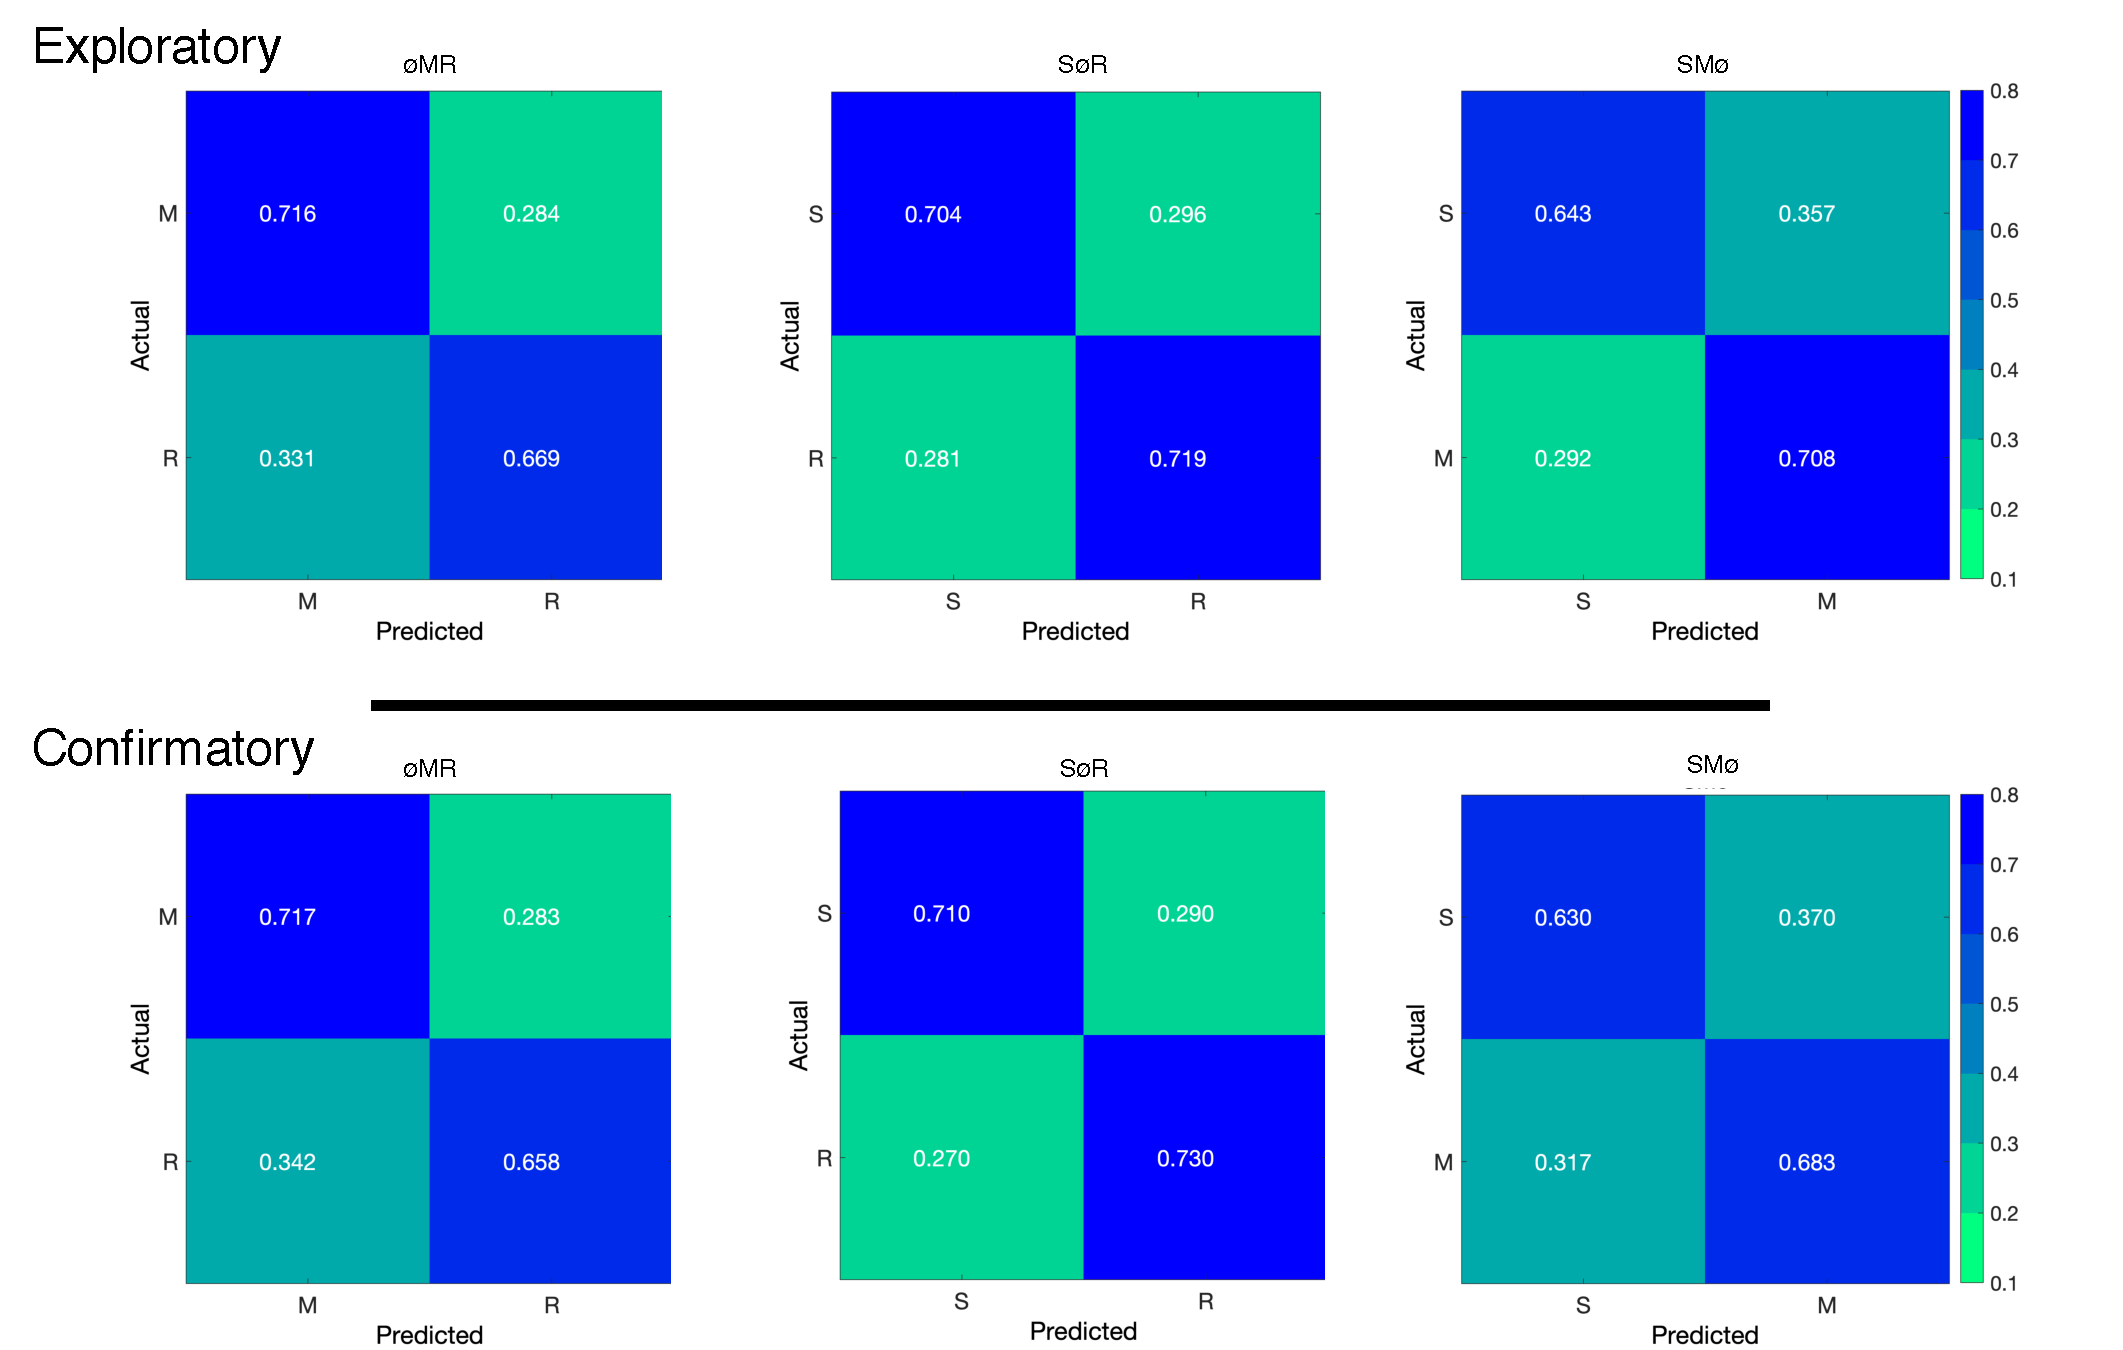
\includegraphics{supplementary_analysis/confusion_matrices/supp_conf_matrices.pdf}
\caption{\label{fig:supp-conf-matrices}The confusion matrices represent the
average classification accuracies for each condition of the timeline
data (S = Search, M = Memorize, R = Rate). The vertical axis of the
confusion matrices represents the actual condition for trial. The
horizontle axis of the confusion matrices represents the condition that
was predicted by the model.}
\end{figure}

Overall, the accuracies for all of the data subsets observed in the
supplementary analysis were higher than the accuracies observed in the
main analysis. Chance accuracy levels for the primary analysis was 33\%,
but because one of the tasks was removed from each element observed in
the supplementary analyses, chance accuracy for these analyses was 50\%.
Given the data analyzed for these supplementary purposes have different
thresholds of chance performance, any conclusions drawn from a
comparison between the primary and supplementary datasets could be
misleading. For this reason, we revisited the results from the primary
analyses and re-calculated the accuracies to be equivalent to a 50\%
chance threshold. The accuracies were recalculated using the following
formula: Accuracy\(_{New}\) = Accuracy\(_{Original}\) /
(Hits\(_{Original}\) + Misses\(_{Original}\)). For example, accuracy for
the Search classification for S\(\varnothing\)R would be calculated with
the following: Search\(_{Hits}\) = Hits\(_{Search}\) /
(Hits\(_{Search}\) + Misses\(_{Search}\)), where Misses\(_{Search}\) is
the ratio of Search trials that were misclassified as Rate.

The re-calculated confusion matrices for each category are presented in
Figure \ref{fig:recalc-conf-matrices}. The general pattern of findings
presented in the re-calculated confusion matrices was the same as the
pattern that can be seen in the supplementary analysis. This is also
true for the pattern of results for the overall accuracies (see Figure
\ref{fig:supp-chance}). In both analyses, the subsets that include the
Memorize trials were classified with lower accuracy than the other data
subsets. Furthermore, a closer look at the confusion matrices shows that
the Memorize conditions were most often confused with the other two
conditions. Because the Memorize condition was mis-classified to a
similar extent when paired with Search or Rate conditions, and these
mis-classifications affected the overall accuracies to a similar extent,
we believe it is likely that there was an increased presence of noise in
the eye movement data for the Memorize trials.

\begin{figure}
\centering
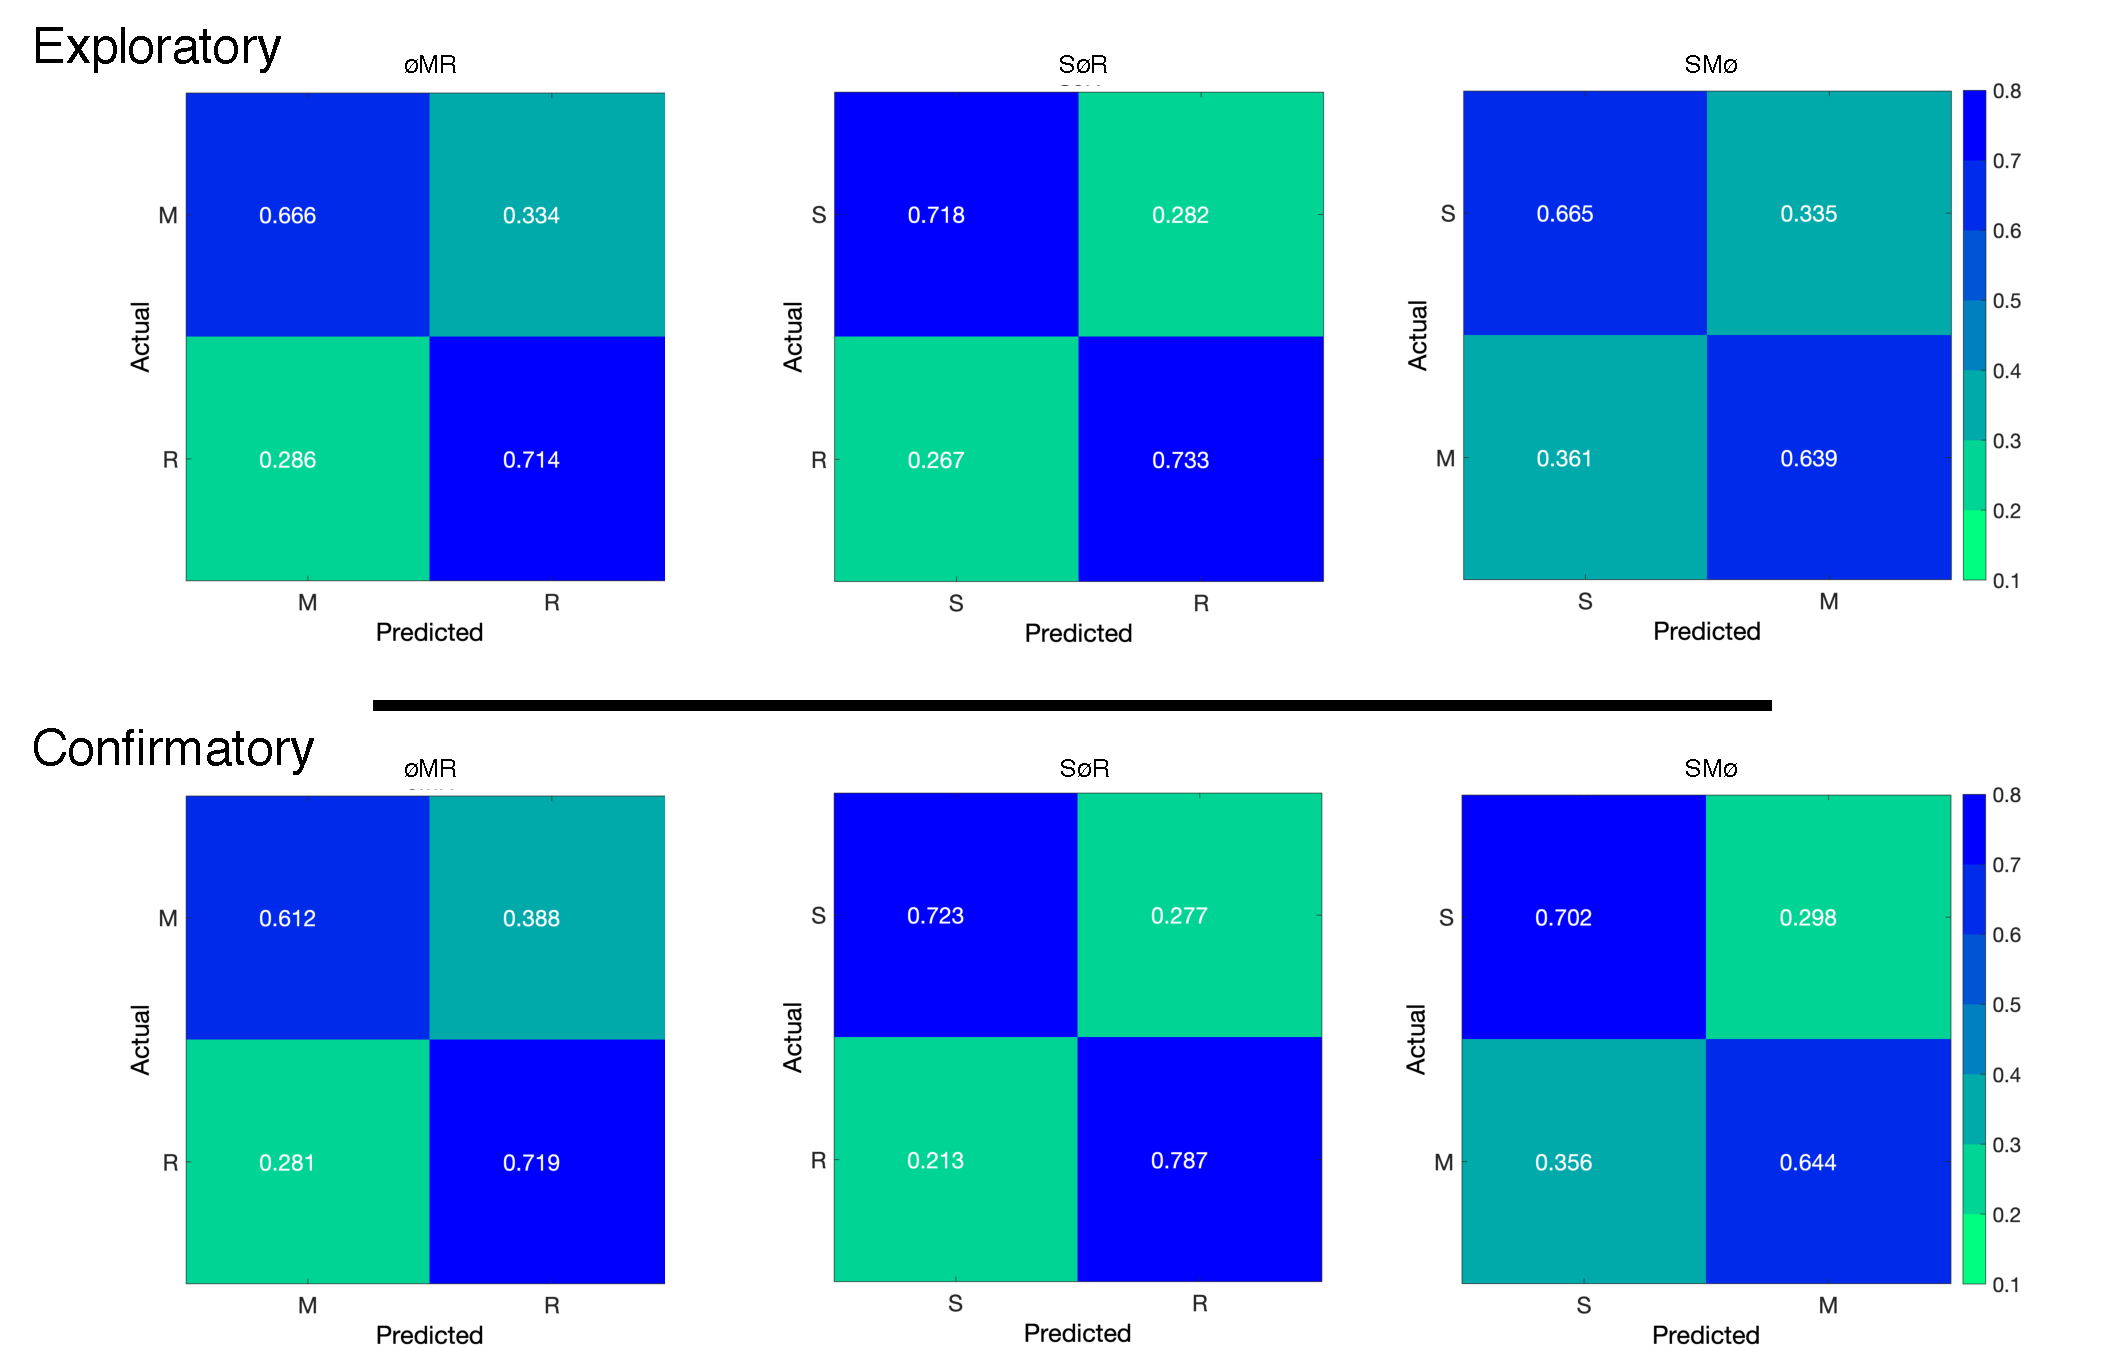
\includegraphics{supplementary_analysis/recalc_orig_accs/confusion_matrices/recalc_conf_matrices.pdf}
\caption{\label{fig:recalc-conf-matrices}The confusion matrices represent a
re-calculation of the classification accuracies for each category from
the primary analysis. This re-calculation is meant to make the
accuracies presented in the primary analysis (chance = 33\%) equivalent
to the classification accuracies presented in the supplementary analysis
(chance = 50\%).}
\end{figure}
\end{appendix}

\end{document}
